\PassOptionsToPackage{table}{xcolor}
\documentclass[twoside, english, draft]{sdqthesis}




%% ---------------------------------
%% | Information about the thesis  |
%% ---------------------------------

%% Name of the author
\author{Niko Benkler}

%% Title (and possibly subtitle) of the thesis
\title{From Monolith to Microservices}

%% Type of the thesis 
\thesistype{Proposal}

%% Change the institute here, ``IPD'' is default
% \myinstitute{Institute for \dots}

%% You can put a logo in the ``logos'' directory and include it here
%% instead of the SDQ logo
% \grouplogo{myfile}
%% Alternatively, you can disable the group logo
% \nogrouplogo

%% The reviewers are the professors that grade your thesis
\reviewerone{Prof. Dr. Ralf H. Reussner}
\reviewertwo{Jun.-Prof. Dr.-Ing. Anne Koziolek}

%% The advisors are PhDs or Postdocs
\advisorone{Dr. Robert Heinrich}


%% Please enter the start end end time of your thesis
%  TODO           \editingtime{xx. Month 20XX}{xx. Month 20XX}

\settitle

%% --------------------------------
%% | Settings for word separation |
%% --------------------------------

%% Describe separation hints here.
%% For more details, see 
%% http://en.wikibooks.org/wiki/LaTeX/Text_Formatting#Hyphenation
\hyphenation{
% me-ta-mo-del
}

%% --------------------------------
%% | Bibliography                 |
%% --------------------------------

%% Use biber instead of BibTeX, see README
\usepackage[citestyle=numeric,style=numeric,backend=biber]{biblatex}
\addbibresource{thesis.bib}


\usepackage[T1]{fontenc}
\usepackage[table]{xcolor}    % loads also »colortbl«
\usepackage{makecell}
\usepackage{adjustbox}
\usepackage{tabularx} % in the preamble
\usepackage{pdflscape}
\usepackage{afterpage}
\usepackage{capt-of}
\usepackage{threeparttable}
\usepackage{graphicx}
\usepackage{pdfpages}


%% ====================================
%% ====================================
%% ||                                ||
%% || Beginning of the main document ||
%% ||                                ||
%% ====================================
%% ====================================
\begin{document}

%% Set PDF metadata
\setpdf

%% Set the title
\maketitle

%% The Preamble begins here
\frontmatter

% TODO wieder rein %% LaTeX2e class for student theses: Declaration of independent work
%% sections/declaration.tex
%% 
%% Karlsruhe Institute of Technology
%% Institute for Program Structures and Data Organization
%% Chair for Software Design and Quality (SDQ)
%%
%% Dr.-Ing. Erik Burger
%% burger@kit.edu
%%
%% Version 1.3.3, 2018-04-17

\thispagestyle{empty}
\null\vfill
\noindent\hbox to \textwidth{\hrulefill} 
\iflanguage{english}{I declare that I have developed and written the enclosed
thesis completely by myself, and have not used sources or means without
declaration in the text.}%
{Ich versichere wahrheitsgemäß, die Arbeit
selbstständig angefertigt, alle benutzten Hilfsmittel vollständig und genau
angegeben und alles kenntlich gemacht zu haben, was aus Arbeiten anderer
unverändert oder mit Änderungen entnommen wurde.}
 
 
%% ---------------------------------------------
%% | Replace PLACE and DATE with actual values |
%% ---------------------------------------------
\textbf{PLACE, DATE}
\vspace{1.5cm}
 
\dotfill\hspace*{8.0cm}\\
\hspace*{2cm}(\theauthor) 
\cleardoublepage

\setcounter{page}{1}
\pagenumbering{roman}

%% ----------------
%% |   Abstract   |
%% ----------------
%% For theses written in English, an abstract both in English
%% and German is mandatory.
%%
%% For theses written in German, a German abstract is sufficient.
%%
%% The text is included from the following files:
%% - sections/abstract

\includeabstract

%% ------------------------
%% |   Table of Contents  |
%% ------------------------
\tableofcontents

\listoffigures
\listoftables

%% -----------------
%% |   Main part   |
%% -----------------

\mainmatter


\chapter{Introduction}
\label{ch:Introduction}
The monolithic software architecture is the traditional pattern to design software, in which functionality is bundled in one single, large application \cite{DataflowDrivenChen}. Although monoliths have their strength, like fast development and simple deployment, they become an obstacle when they grow in size and become more complex \cite{infoq}. Incomprehensible code structure makes it difficult to add functionality, fix bugs and enable new software engineering approaches like Continuous Delivery and Continuous Deployment \cite{cd}. 
Besides, the rise of cloud computing demands a new architecture that can fully exploit the rich set of features given by the cloud infrastructure \cite{MigratingCloud}. \\
Inspired by service-oriented computing, the microservice architecture is about to become a promising alternative to overcome the shortcomings of centralized, monolithic architectures and consequently gains popularity in both, academia and industry \cite{ObjectAwareAmiri}. Benefits like the increase of agility, resilience or scalability \cite{FunctionalDecompositionHeinrich}, the ability to use different technology stacks and independent deployment \cite{interfaceAnalysisBaresi} and the efficient resource utilization in cloud environments \cite{MigratingCloud} explain the usage of microservice-based applications by big companies like Google, Netflix \cite{DevOps}, Amazon, eBay \cite{DataflowDrivenChen} and Uber \cite{FunctionalDecompositionHeinrich}. \\
This chapter presents the motivation for the topic and the contributions of this thesis.


\section{Motivation}
\label{sec:Introduction:Motivation}
Monolithic software applications develop over time and become more and more complex. The software structure becomes highly coupled and hard to maintain \cite{MigratingTowardsSurvey}. To tackle this issues, software engineers started to decompose their system into modules and provide the functionality over the network as Web Services \cite{ServiceCutter}. The so-called \textit{Service-oriented Architecture} (SOA) provides logical boundaries between the different software modules to address the design challenge of distributed systems. Nevertheless, Baresi et. al state that the boundaries between modules in SOA are too flexible and the application results in "a big ball of mud" \cite{interfaceAnalysisBaresi}. Microservices make these boundaries physical as each service runs in its own process and only communicates with other services through well-defined lightweight mechanisms like REST \cite{FunctionalDecompositionHeinrich}. Chen \textit{et al}. consider the microservice architecture as a particular approach for SOA \cite{DataflowDrivenChen}. Others look at it as an evolution of SOA with differences in service reuse \cite{interfaceAnalysisBaresi} or consider it to be the "contemporary incarnation of SOA" combined with modern software engineering practices like Continuous Deployment \cite{ServiceCutter}. There is no consensus about the relationship between microservices and SOA but they both share common characteristics.
The microservice architecture has many advantages over the monolithic style. Sec.\ref{sec:background:microservices} elaborates the main aspects of microservices, including several benefits. Netflix, for instance, is able to cope with one billion calls a day to its video streaming API, by migrating their monolithic system to a highly flexible, maintainable and scalable microservice architecture \cite{DataflowDrivenChen}. Consequently, moving existing applications to a microservice landscape is an upcoming philosophy in academia and industry \cite{ObjectAwareAmiri}. Besides the migration of existing system towards a microservice architecture, many greenfield systems are already designed using the microservice architecture.\\
Nevertheless, decomposing a (existing) system in loosely coupled, fine-grained and independent microservices is a time consuming task that requires tedious manual effort \cite{ServiceCutter} and is technically cumbersome \cite{HeuristicsAlwis}. So far, it is done mainly intuitively and relies on the experience of software architects and system designers. Hence, a formal approach to identify microservices is required. 


\section{Research Questions and Contributions}
\label{sec:Introduction:ResearchQuestions}
The microservice architecture is a fast rising approach to structure a system as a collection of highly cohesive but loosely coupled and independent services. Large applications are decomposed into small, independent microservices where each service can be independently scaled and deployed. 
\\
However, one of the biggest problem in designing a microservice architecture is to decompose an application into a suite of small services while keeping them loosely coupled and highly cohesive. This challenging task is also known as \textit{microservice identification} \cite{ObjectAwareAmiri}. \\
Baresi \textit{et al.} state that a "proper" microservice identification defines how a system will be able to evolve and scale \cite{interfaceAnalysisBaresi}. Others claim, that finding the optimal microservice boundaries \cite{ClassificationOfRefactoring} and service granularity  \cite{ArchitecturalMetaModelling} is the key design decision to fully leverage the benefits of microservices. 
\\
So far, the partition is performed mainly intuitively based on the experience and know-how of experts that perform the extraction. Hassan \textit{et al.} criticise a lack of systematic approaches to reduce the complexity of the extraction process \cite{ArchitecturalMetaModelling}. Extracting microservices from monoliths or design a larger greenfield application as microservice-based system therefore requires tedious manual effort and can be very costly \cite{FunctionalDecompositionHeinrich} \cite{ExtractionMazlami}. In the following, we present Research Questions (RQ) to tackle the issue of microservice identification. They are general and do not restrict the application area to a single system type:


\vspace{1cm}
\par
\begingroup
\leftskip=1cm
\rightskip=1cm

\noindent
\textbf{RQ1: How to identify microservices based on the system specifications?}

\vspace{0.5cm}
\noindent
The research question can be further divided into more specific sub-questions, where the first question covers the literature research, the second one addresses the construction of a new approach and the last one deals with the evaluation.

\vspace{0.5cm}
\noindent
\textbf{RQ1.1: Which is an appropriate strategy to decompose a system into microservices?}

\vspace{0.5cm}
\noindent
To identify possible strategies, a literature research is conducted. Suitable strategies and approaches are compared based on criteria identified in the literature research.
\vspace{0.5cm}

\noindent
\textbf{RQ1.2: What formal approach can be constructed to identify possible microservices without detailed know-how and manual effort?}

\vspace{0.5cm}
\noindent
To that end, the most promising strategy identified in RQ1.1 is used as basis. Thereupon, a formal approach is elaborated that aims to reduce the complexity and manual work that has to be done when identifying microservices.
\vspace{0.5cm}


\noindent
\textbf{RQ1.3: What is the accuracy of the approach?   }

\vspace{0.5cm}
\noindent
Research question RQ1.3 is tackled by applying the approach to the Common Component Modelling Example (\textit{CoCoME}). The subsequent system decomposition is evaluated by comparing the identified microservices with two other approaches: First, Tyszberowicz \textit{et al.} \cite{FunctionalDecompositionHeinrich} provide a decomposition of CoCoME based on their approach. Second, we identified and implemented a microservice-based version of CoCoME manually. 

\vspace{0.5cm}



\endgroup
\vspace{1cm}







\section{Thesis Outline}
\label{sec_Introduction:ThesisOutline}
The proposal is structured as follows:


\begin{itemize}
	\item  Chapter \ref{ch:background} presents the background information on monolithic software architecture and microservice-based architecture. For the latter one, benefits and challenges are elaborated. Further this chapter introduces a specific use case notation and the business process modelling language \textit{BPMN.}
	\item Chapter \ref{ch:CoCoME} introduces the running example \textit{CoCoME} that is used to apply and evaluate the approach. Special attention is given to the system specifications.
	\item Chapter \ref{ch:StateOfTheArt} outlines the current state of the art concerning microservice identification. First, the process of literature review is presented. Second, the most promising strategies and approaches are described and further compared using adequate criteria.
	\item Chapter \ref{ch:Solution} proposes a graph-based approach to identify microservices. The process is divided in several steps, where each step is presented in a separate section.
	\item Chapter \ref{ch:SolutionApplication} applies the approach to the running example. All intermediate results will be presented as well as a decomposition of \textit{CoCoME} into microservices.
    \item Chapter \ref{ch:Evalutation} evaluates the approach. First, the evaluation method is presented. Second, two reference sets are introduced which are used to evaluate the result of the previous chapter. Finally, the threats to validity are presented.
    \item The thesis is concluded by chapter \ref{ch:Conclusion}, the main outcomes are summarized and discussed. Eventually, the limitations and future work are presented.
    

\end{itemize}












\chapter{Background}
\label{ch:background}
This chapter introduces and compares the monolithic software architecture and the microservice architecture. Further, benefits and challenges of the microservice architecture are outlined. Also, it introduces a well known and established use case notation technique and a standardized notation to capture business processes.



\section{Monolithic Software Architecture}
\label{sec:background:monolith}
The monolithic software architecture is a well-known and the most widely used pattern for Enterprise Applications, which usually are built in three main parts (top to bottom): The client-side user interface (Tier 3), the server-side application that contains the entire business logic (Tier 2) and the persistence layer handling the database access (Tier 1). Fig. \ref{fig:architekturMonolithVsMS} illustrates the architectural difference between a standard three tier application and a exemplary microservice-based architecture. The server-side application - \textit{the monolith} - is a single unit and deployed on one application server \cite{infoq}. The software structure, if well defined, is composed of self-contained modules (i.e. software components), where each module consists of a set of functions \cite{HeuristicsAlwis}.
The monolith implements a complex domain model, including all functions, many domain entities and their relationships.
For small applications, this approach works relatively well. They are simple to develop, test and deploy \cite{FunctionalDecompositionHeinrich}. Fast prototyping is supported by current frameworks and development environments (IDEs), which are still oriented around developing single applications \cite{infoq}.
\\
But once they grow in size, they become exceedingly difficult to understand and hard to maintain without reasonable effort \cite{FunctionalDecompositionHeinrich} \cite{ClassificationOfRefactoring}. A complex and large code base prevents a fast addition of new features and makes the application risky and expensive to evolve \cite{TowardsTechnique}.
Alterations to the system, even though they might be small, result in a redeployment of the whole monolith application due to its nature being a single unit \cite{FunctionalDecompositionHeinrich}. Moreover, it is difficult to adopt newer technologies without rewriting the whole application, as monoliths are build on a specific technology stack \cite{infoq} \cite{ExtractionMazlami}.\\
Scaling is only possible by duplicating the entire application, namely \textit{horizontal scaling}. Consequently, large portions of the infrastructure remain unused, if only parts of the application need to be upscaled or even used \cite{EnticeApproach} \cite{MigratingTowardsSurvey}. \\
Rui Chen describes the shortcomings of monolith as follows: "Successful applications
are always growing in size and will eventually become a
monstrous monolith after a few years. Once this happens,
disadvantages of the monolithic architecture will outweigh
its advantages" \cite{DataflowDrivenChen}.



\section{Microservices}
\label{sec:background:microservices}
M.Fowler and J.Lewis describe the microservice architectural style as "an approach to developing a single application as a suite of small services, each running in its own process and communicating with lightweight mechanisms, often an HTTP resource API"\cite{Fowler}.

\begin{figure}[t]
	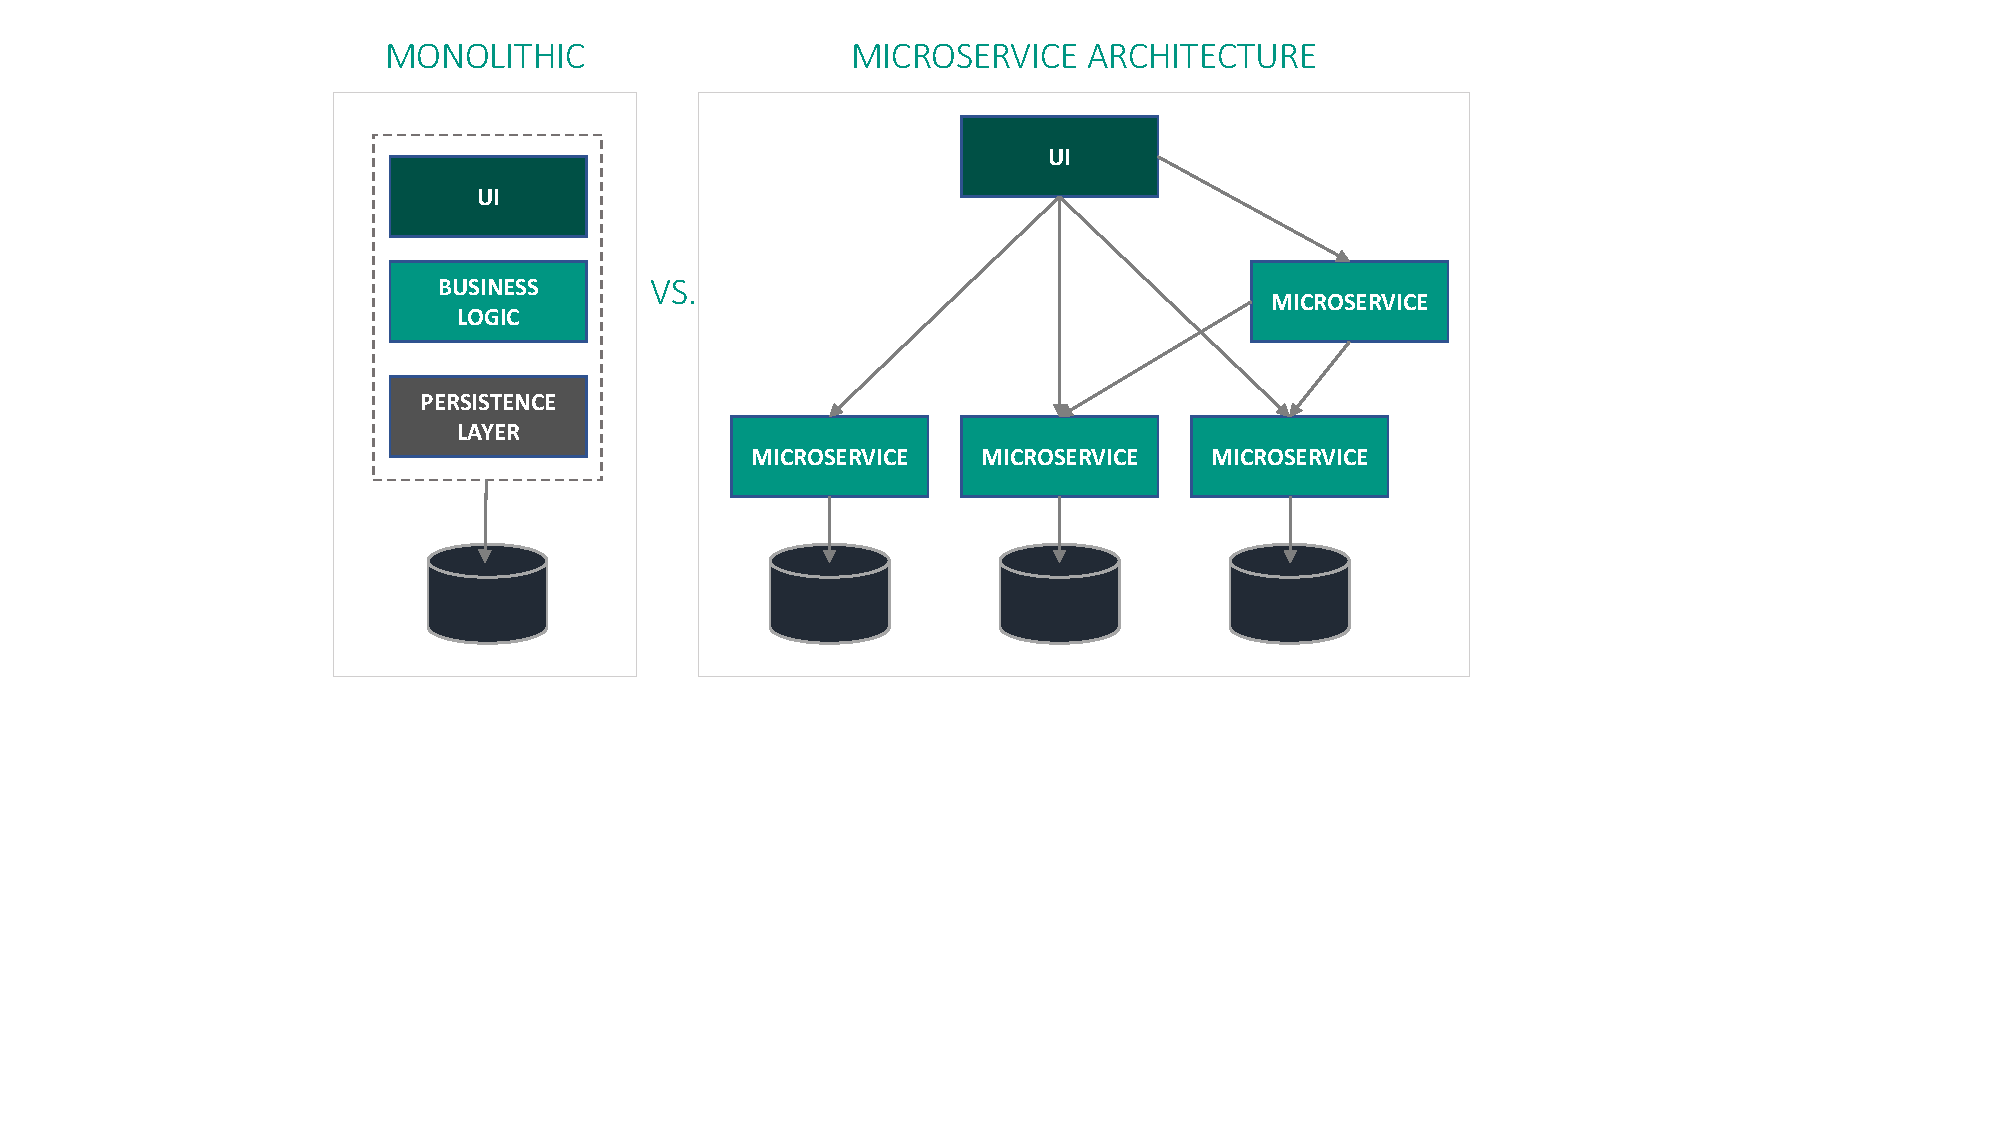
\includegraphics[width=\textwidth, trim={5cm 8cm 8cm 3cm}]{img/Architektur.pdf}
	\caption{Monolithic vs. Microservice Architecture}
	\label{fig:architekturMonolithVsMS}
\end{figure}

\subsection{Definition}
Yet, the term microservices is not formally defined in academia. A popular definition of microservices is  "a collection of cohesive and loosely coupled components, where each service implements a business capability"\cite{ObjectAwareAmiri}.
Amiri introduces three principles upon which the architecture is build: \textit{Bounded Context, Size, Independence} \cite{ObjectAwareAmiri}. \\
The first principle is about related functionality, that is combined in a single business capability - the  \textit{bounded context} \cite{FunctionalDecompositionHeinrich}. Each capability is implemented by one microservice. 
The \textit{Size} of a microservice is defined by the number of features it provides (namely bundled functional capabilities)  \cite{WorkloadbasedClustering}. There is no consensus about the "proper" size of a microservice \cite{DomainEngineeringMunezero}, but several guidelines exists: Services should focus on one business capability only \cite{ObjectAwareAmiri}. Others state, that the size of a microservice should not exceed a level, where it cannot be rewritten within six weeks \cite{WorkloadbasedClustering}. However, the sizes vary from system to system \cite{FunctionalDecompositionHeinrich} and even different sizes for each microservice in a specific system are possible \cite{DomainEngineeringMunezero}. The bottom line of \textit{Independence} is in Amiri's description of microservices as "a collection of high cohesive and loosely coupled components" \cite{ObjectAwareAmiri}. High cohesive services implement a relatively independent piece of business logic (at the most one business capability). Further, microservices should hardly depend on each other, which is the idea of being loosely coupled \cite{DataflowDrivenChen}.\\
Communication between microservices is achieved by lightweight message passing mechanisms such as \textit{REST}. Each service exposes a well defined interface (\textit{API}) with endpoints that provide information using standard data formats \cite{FunctionalDecompositionHeinrich}. 
The design of microservices mainly follows the \textit{Single Responsibility Principle (SRP)}: Each service should not have more than one reason to change \cite{TowardsUnderstandingEvolution}. The SRP mainly corresponds to the idea of not implementing more than one business capability.
The following covers the benefits and challenges of the microservice architecture.





\FloatBarrier

\subsection{Benefits}
\textbf{Fast and Independent Deployment} \\
As a matter of fact, each microservice is deployed independently \cite{interfaceAnalysisBaresi}. Changes to the code do not result in a full redeployment of the entire application \cite{FunctionalDecompositionHeinrich}. Consequently, software developers are able to react much quicker to changes in business requirements. This includes an acceleration in error correction. Per contra, any changes in a monolithic code base require a time consuming build of a new version and the redeployment of the entire application \cite{Fowler}. \\

\noindent
\textbf{Availability, Resilience and Fault Isolation} \\
Microservices are designed to operate independently of each other and to tolerate failure of services \cite{Fowler}. Large parts of the application remain unaffected of partly failures and the availability of the system is, at least partly, guaranteed. Monolithic application do not provide this type of fault isolation. If a failure occurs, the whole application remains unavailable as it is usually running in a single process \cite{ExtractionMazlami}. \\
 
\noindent
\textbf{Scalability and Resource Utilisation} \\
Small and independent microservices allow more fine-granular horizontal scaling \cite{WorkloadbasedClustering}. Single services can be duplicated to cope with changing workload during runtime \cite{DataflowDrivenChen}. Thus, dynamic (de-)allocation of resources on demand prevent infrastructure from being idle \cite{HeuristicsAlwis}. Scaling monoliths can only be attained by duplicating the entire application, leaving resources unused \cite{ClassificationOfRefactoring}. Further, each microservice is deployed on the best suitable infrastructure for its needs, allowing a more efficient system organization \cite{infoq}. \\

\noindent
\textbf{Improved Productivity} \\
In traditional software development, teams are divided based on their expertise: Database architects, UI-developers and server-side engineers, resulting in a three-tiered application (cf. Sec.\ref{sec:background:monolith}). Additionally, software engineers are responsible for the development only. Deployment is part of the operations team. This team structure results in high communication overhead and slows down the productivity \cite{Mazlami}. \\
In contrast, microservices are organized around business capabilities and require cross-functional, independent teams \cite{ObjectAwareAmiri}. Each team has the full range of skills required for the end-to-end realization of a microservice, including UI-development, database architecture, back-end engineers and project management. 
This minimizes the communication and interaction between the teams and thus, speeds up the productivity. Ultimately, microservices enable a more agile flow of development and operation \cite{ClassificationOfRefactoring}, also referred as \textit{DevOps}. 
\\


\noindent
\textbf{Neutral development technology} \\
Microservices are highly decoupled from each other, as they use standardized and lightweight communication mechanisms such as REST \cite{FunctionalDecompositionHeinrich}. Microservices can be realized using different programming languages, technologies and even deployment environments \cite{DataflowDrivenChen}. Developers are consequently not longer limited to use a single technology for the whole application. They can choose the most appropriate technology for each particular business problem or try out some new technology without rewriting the whole application \cite{ServiceCutter} \cite{TowardsTechnique}. 
 



\subsection{Challenges}
The previous section provides a vast amount of benefits that come with microservices. However, microservices are not the panacea of software engineering. System developers have to face challenges that can mitigate the benefits as described previously. The challenges are described in the following. \\ 

\noindent
\textbf{Expensive Communication}\\
Microservice use network protocols such as \textit{HTTP} to communicate with each other. Compared to standard, inter process communication (\textit{IPC}) as used in monoliths, remote procedure calls a more expensive \cite{SystematicMappingStudyMicroservice}. As a consequence, applications experience a decrease in performance as network communication is generally slower than \textit{IPC}.\\

\noindent
\textbf{Technical Challenges}\\
Microservices require a high degree of infrastructure automation \cite{MigratingTowardsSurvey}. The benefits of fast and independent deployment cannot be utilized, if it has to be done manually. Dynamic (de-)allocation of resources when scaling individual microservices need a well defined and structured cloud environment \cite{MigratingCloud}. 
Besides, the distributed microservice landscape complicates the logging mechanisms and performance monitoring \cite{SystematicMappingStudyMicroservice}. Traditional centralized logging, as it is used in monolithic applications, is not longer applicable. Instead, a careful aggregation system to gather logging and monitoring data from each service is required.\\

\noindent
\textbf{Organizational Challenges}\\
The microservice approach needs the establishment of cross-functional teams \cite{Fowler}. Adopting \textit{Continuous Practices}, such as \textit{Continuous Deployment}, are essential for the success of a profitable microservice architecture. Therefore, closer collaboration between development teams, operational staff and management has to be established. In summary, a costly and time consuming restructuring process of the entire organization is required \cite{NikoProseminar}. \\



\noindent
\textbf{Data Consistency}\\
Distributed systems need to share data. Heinrich et al. propose two concepts for the database architecture \cite{FunctionalDecompositionHeinrich}: The first concept applies the basic idea of the microservice approach, as it splits the database into several parts. Each microservice has its own database which manages the entities that belong to the corresponding bounded context. Higher speed and horizontal scaling are facing data consistency issues. Data needs to be synchronized which leads to inconsistency, if services are unavailable. The second concept is about sharing a single database. This approach overcomes the issue of consistency, as data is stored centrally. But sharing results in a loss of independence. Scaling can only be achieved through replicating the whole database. Research revealed, that the first concept is preferred \cite{FunctionalDecompositionHeinrich}. \\



\noindent
\textbf{Decomposition}\\
Decomposing a system into microservices is a very complex task that requires experienced system architects and domain experts \cite{Fowler}. It is irrelevant whether an existing system is decomposed into microservices or whether a new system is designed as a microservice-based application. The effort is very high in both cases.\\
Identifying the right granularity of microservice is one of the key issues. Too fine grained services cause inefficiency due to a high amount of expensive inter-service calls \cite{DomainEngineeringMunezero}. Developing the basic communication infrastructure adds additional complexity and slows down the initial developing process \cite{infoq}. \\



\section{Use Cases}
\label{sec:PrepApproach:UC}
Use Cases are a widely adopted technique to document software system requirements. Generally, they describe the interaction between actors (usually system users) and the software system itself. In this thesis, use cases are provided as semi-structured tables (following the notation presented by Cockburn et al. \cite{Cockburn}). \\ An example is given in Table \ref{tab:exampleUseCase}: Each use case has a unique identifier and a short description, followed by necessary preconditions and a trigger that causes the execution. The standard process is the main part and describes the success steps of the Use Case. Extensions provide additional information like alternatives or exceptional processes that occur in case of an unsuccessful step. 




\begin{table}[!h]
	\centering
	\begin{tabularx}{\textwidth}{|l||X|}
		\hline
		UC 5 & Show Stock Reports \\ 
		\hline
		Brief Description &  The opportunity to generate stock-related reports is provided
		by the Trading System. \\
		\hline
		Precondition & The reporting GUI at the Store Client has been started. \\
		\hline
		Trigger & The Store Manager wants to see statistics about his store. \\
		\hline
		Postcondition & The report for the Store has been generated and is displayed on
		the reporting GUI. \\
		\hline 
		Standard Process &
		
		1. The Store Manager enters the store identifier and presses the button Create
		Report.  \\
		& 2. A report including all available stock items in the store is displayed. \\  
		\hline
		Extensions & (none) \\ \hline
		
		
	\end{tabularx}
	\caption{Example Use Case in Tabular Form, Source: \cite{CoCoMEOld}}
	\label{tab:exampleUseCase}
	
\end{table}

\noindent
Besides being a widely adopted technique to specify system requirements, the textual use case notation is understandable without further technical knowledge. Neither previous knowledge in specific graphic notations like UML, nor the capability to create a complex domain model is necessary. Consequently, all sort of stakeholders (non-technical and technically experienced) are capable to provide the necessary information in terms of use cases. \\
However, the transformation into business models as presented in Sec.\ref{sec:PrepApproach:TransformUCtoBPMN} is not always trivial and requires some manual effort to produce high quality business processes. Nevertheless, it is necessary as the system requirements of the running example are given in form of textual use cases.





\section{Business Process and Model Notation}
\label{sec:PrepApproach:BPMN}
The Business Process and Model Notation (BPMN) is a graph oriented language to describe business processes. Originally, BPMN was designed to describe activities and their control flow dependencies only \cite{VisualizeBPMN}. Since the introduction of BPMN 2.0, it is possible to model the data needs and the data results of activities \cite{OMG}. Consequently, BPMN is capable to express the control flow and to approximate the data flow of business processes \cite{DataFlowErrorBPMN}. In the remainder, we use BPMN and BPMN 2.0 interchangeably. \\
BPMN is easy-to-use, powerful and widely adopted in academia and industry. Hence, BPMN is a suitable approach to extract the implicitly given data flow and control flow in the use case description. Sec.\ref{sec:PrepApproach:TransformUCtoBPMN} introduces a formal approach to generate BPMN processes from use case sets. Next, the BPMN 2.0 process definition is shortly introduced:

%"l, b, r, t"
\begin{figure}[h!]
	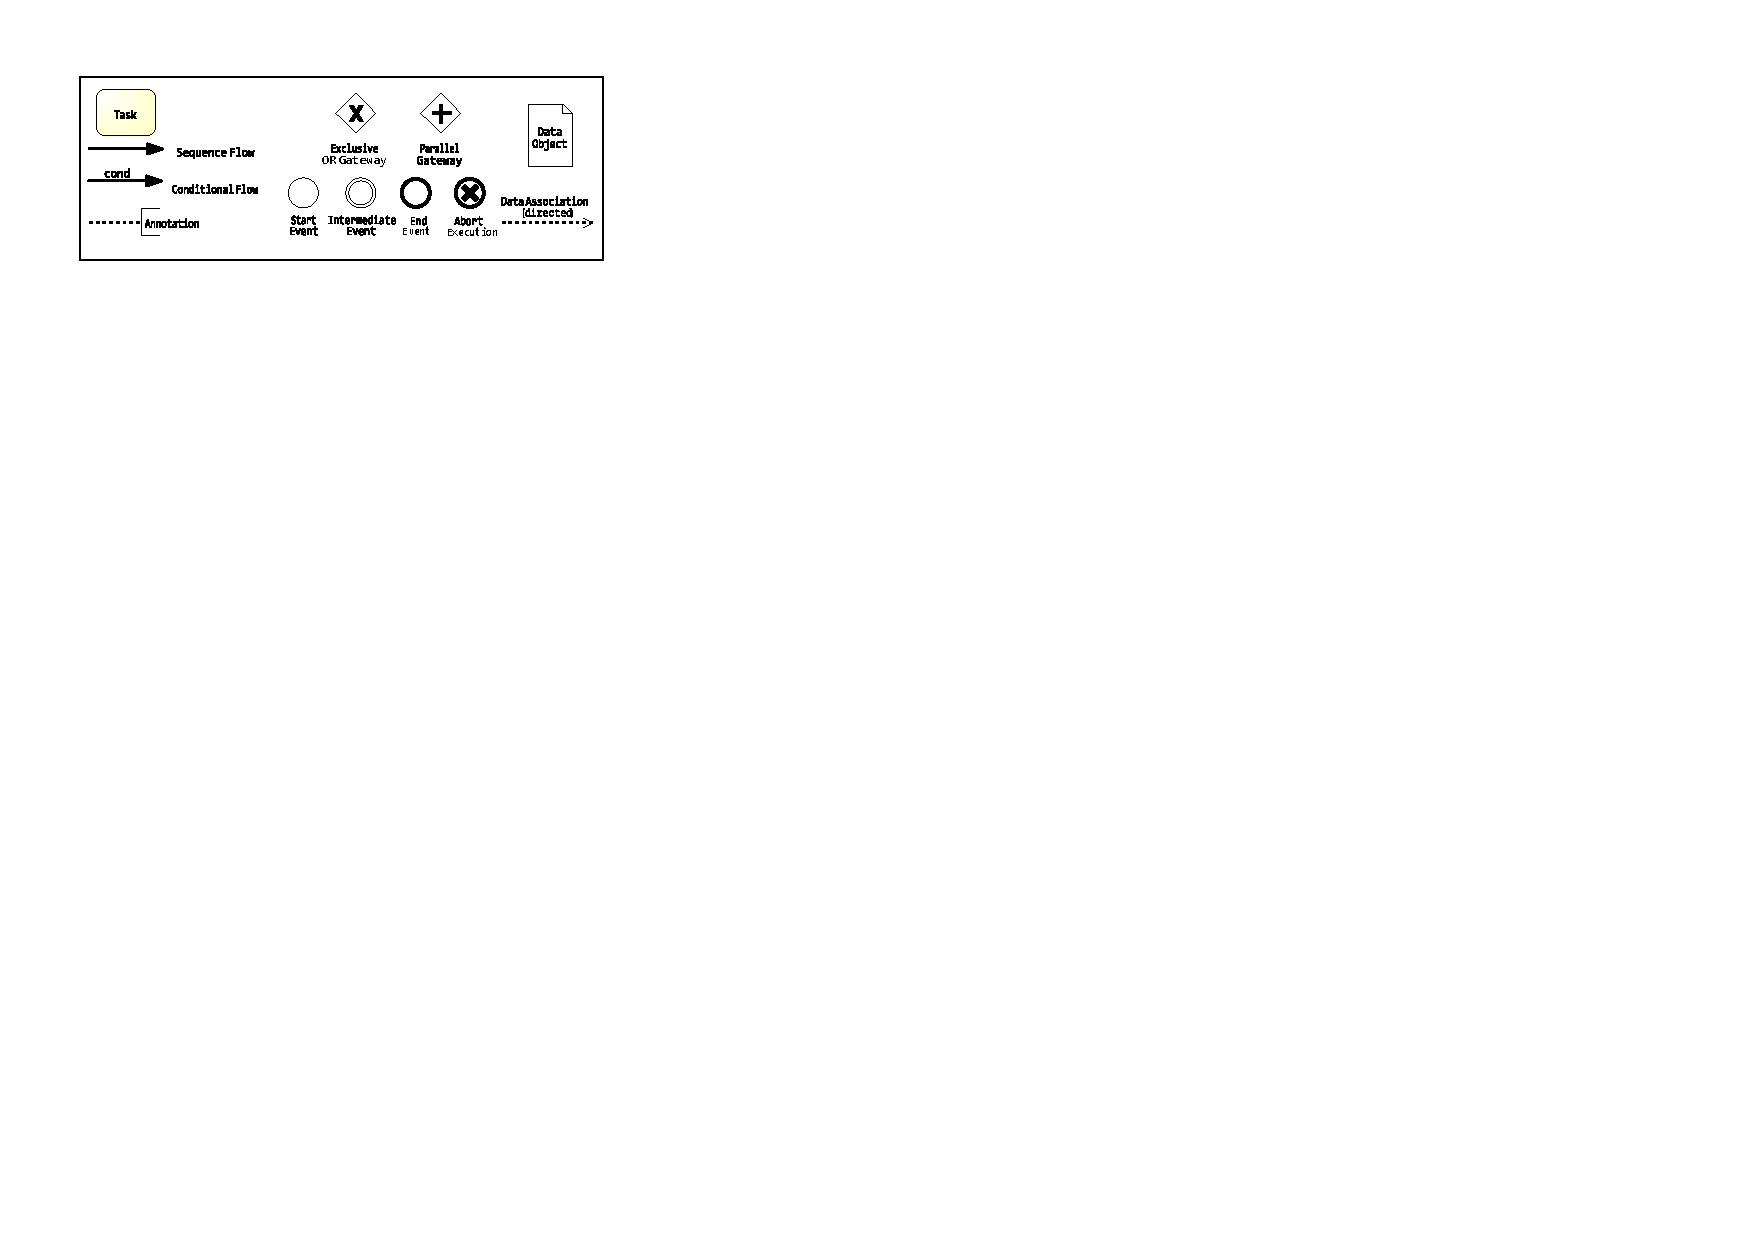
\includegraphics[width=\textwidth, trim={1cm 16.8cm 19.5cm 1cm}]{img/Overview.pdf}
	\caption{BPMN Notation (Subset)}
	\label{fig:BPMNSubset}
\end{figure}

\noindent
Fig.\ref{fig:BPMNSubset} presents the subset of BPMN symbols, that is required for the approach presented in this thesis \footnote{The entire specification is available at https://www.omg.org/spec/BPMN/2.0/}. Control flow activities are modelled as atomic \textit{Tasks} and connected through \textit{Sequence Flow Arcs}. \textit{Conditional Flow Arcs} integrate decision points into the control flow. Navigation decisions are based on the conditions related to the individual arcs. Such decision point are the \textit{Exclusive Or Gateway} and the \textit{Parallel Gateway}. Regarding the first one, if one of the incoming flows is triggered exactly one outgoing flow is activated based on the condition. For the latter, all outgoing flows are activated as soon as all of its incoming flows are activated. Each BPMN process starts with a \textit{Start Event} and ends with an \textit{End Event}. In case of several branches (due to Gateways), stop events need to be placed to each end. \textit{Intermediate Events} mark any other events that occur during the process. The trigger for an event is modelled using the \textit{Annotation} symbol. The \textit{Abort Execution Event} extend the \textit{End Event} and marks the error-prone end of a business process. \\
When it comes to data, each \textit{Task} may or may not require and/or produce data. Directed \textit{Data Association Arcs} provide the opportunity to model data needs and data results. In case a task requires data, the corresponding \textit{Data Objects} are connected to the task with the arrowhead attached to the task. Producing data works in the opposite direction. \\









\chapter{CoCoME}
\label{ch:CoCoME}

\section{Introduction to CoCoME}
\label{sec:CoCoME:Introduction}


\chapter{State of the Art}
\label{ch:StateOfTheArt}
This chapter outlines the current state of the art regarding microservice identification.  Sec. \ref{sec:StateOfTheArt:LiteratureReview} presents the search strategy and several existing approaches (Table \ref{tab:overviewLiterature}) that deal with the identification of microservices. Thereupon, the approaches are further explained and finally compared on the basis of several criteria.

\section{Literature Review}
\label{sec:StateOfTheArt:LiteratureReview}
The approaches mentioned in table \ref{tab:overviewLiterature} are the result of an extensive literature research which was conducted using the digital libraries IEEE \footnote{http://ieeexplore.ieee.org }, ACM \footnote{http://portal.acm.org} and SpringerLink \footnote{http://www.springerlink.com }. The web search enginge Google Scholar \footnote{http://scholar.google.com} provided further approaches and general information. \cite{FunctionalDecompositionHeinrich} was provided by the supervisor of this thesis and \cite{ServiceCutter} was cited by various approaches, including \cite{interfaceAnalysisBaresi}. The following search string was used:

\begin{centering}
{\itshape
   ["identify" OR "identification" OR "migrating" OR "monolith" OR "decomposition" OR "decompose monolith"
  	OR "decompose"] AND  "microservice"  \\
  	   OR \\  "microservice"  AND ["identification" OR "transformation" OR "refactor"]
}
 
   
\end{centering}

\noindent
Table \ref{tab:overviewLiterature} presents the 8 most promising approaches regarding the criteria mentioned in table //TODO!!!!!!. Now, a short introduction to each approach is given.




\begin{table}[h!]

\centering
     
	
	 \rowcolors{2}{gray!25}{white}
	\begin{tabularx}{\textwidth}{lXXlX}
		\rowcolor{gray!50}
		Link & Titel & Author   & Origin & Search String  \\
		
		\rowcolor{gray!50}
		& & (Year) & & \\
		
		\cite{ExtractionMazlami} & Extraction of Microservices from Monolithic Software Architectures  & G. Matzlami et. al. (2017) & Google Scholar&  {\itshape microservice identification }  \\
		
		
		\cite{ObjectAwareAmiri} & Object-Aware Identification of Microservice & M. J. Amiri (2018) & IEEE & \textit{identification microservices}\\\
		
		\cite{interfaceAnalysisBaresi} & Microservices Identification Through Interface Analysis & L. Baresi et. al. (2017)& SpringerLink & \textit{microservice identification}\\
		
		
		
		 
		 \cite{FunctionalDecompositionHeinrich}& Identifying Microservices Using Functional Decomposition & S. Tyszberowicz et. al. (2018) & \textit{provided} & \textit{n/a} \\
		 
		 \cite{DomainEngineeringMunezero} & Partitioning Microservices: A Domain Engineering Approach & I. J. Munezero et. al. (2018) & ACM & \textit{partition microservices}\\
		 
		 
		 \cite{DataflowDrivenChen} & From Monolith to Microservices: A Dataflow-Driven Approach & R.Chen et. al & IEEE & monolith microservice \\
		 
		\cite{HeuristicsAlwis} & Function-Splitting Heuristics for Discovery of Microservices in Enterprise Systems & A. De Alwis et. al. (2018 )& Google Scholar & identify microservices \\
		
	\cite{ServiceCutter} & 	Service Cutter: A Systematic Approach to Service Decomposition& M. Gysel et. al. (2016) & \cite{interfaceAnalysisBaresi} & \textit{n/a} \\
	
	\end{tabularx}
	\caption{List of authors and approaches}
	\label{tab:overviewLiterature}
\end{table}


\clearpage





\section{Approaches}


\noindent
\textbf{Extraction of Microservices from Monolithic Software Architectures   } \\
The approach presented in \cite{ExtractionMazlami} is a class based extraction model, that uses (meta-)information of a version control system \textit{(VCS)} such as Git\footnote{https://github.com/} to identify microservices. The approach is divided in two phases: The \textit{Construction Phase} and the \textit{Clustering Phase}.
Starting with a given code base, the approach uses three different coupling strategies and the information provided by the \textit{VCS} to transform the monolith into a weighted graph. Here, the nodes represent classes, and the edges have weights according to the chosen coupling strategy. In the second phase, a clustering algorithm determines possible microservices (each cluster is a microservice candidate). \\

\noindent
\textbf{Object-Aware Identification of Microservice  } \\
\cite{ObjectAwareAmiri} identifies microservices from business processes, using the widely known \textit{Business Process and Model Notation (BPMN)}. The activities in a business process represent functionality in the system. They also perform read and write operations on data objects. The goal is to identify microservices by using the structural and data object dependencies of the business processes. Therefore, the author proposes a clustering technique


\cite{ObjectAwareAmiri} uses clustering based on structural dependency and data object dependency. The system is modelled 





The approach models a system as a set of business processes using the well known graphical representation 
\noindent
\textbf{Microservices Identification Through Interface Analysis   } \\


\noindent
\textbf{Identifying Microservices Using Functional Decomposition  } \\


\noindent
\textbf{Partitioning Microservices: A Domain Engineering Approach } \\


\noindent
\textbf{From Monolith to Microservices: A Dataflow-Driven Approach } \\

\noindent
\textbf{Function-Splitting Heuristics for Discovery of Microservices in Enterprise Systems  } \\


\noindent
\textbf{Service Cutter: A Systematic Approach to Service Decomposition  } \\




\chapter{Solution Overview}
\label{ch:SolutionOverview}
This chapter provides the solution overview to tackle the issue of microservice identification. Basically, approaches support two types of initial situations: They either conduct the extraction of microservices from existing monolithic systems or they are based on microservice greenfield development. In this thesis, the extraction process is based on the pre-existing system requirements of the case study. Therefore no existing implementation is used and consequently, the presented approach is to be classified as greenfield method.\\
This thesis proposes a formal, graph-based microservice identification approach using clustering techniques and facets of structural and data dependencies extracted from control flow and data flow. The approach is mainly inspired by Amiri's  work on \textit{Object-aware Identification of Microservices}. Hereafter, the approach \cite{ObjectAwareAmiri} is shortly introduced as a solution to \textbf{RQ1}. Sec.\ref{sec:solutionOverview:Contributions} suggests the improvements that form the basis of the approach proposed by this thesis \textbf{(RQ2)}.


\section{Basic Concept}
\label{sec:solutionOverview:basicConcept}
Basically, the identification process is performed from the business process point of view. A business process is a set of activities where each activity represents a functionality within the system in order to achieve a business goal. To organize a system as suite of small and independent microservices, the business processes are decomposed into fine-grained, cohesive and loosely coupled components where the activities are distribute among those components and each of them represents a microservice.\\



\subsection{Available Extraction Strategy}
\label{sec:solutionOverview:basicStrategy}
The partitioning process is based on the structural dependency of the activities and furthermore based on the data object dependencies regarding the read and write operation the activities perform on data objects. To promote the property of high cohesiveness, two activities are more likely to be partitioned into the same microservice if they are close or even directly connected through an edge. Besides, it is desirable to partition activities into the same microservice with similar data access . \\
Technically, the activities are represented by \textit{BPMN}\footnote{Business Process Model an Notation} business processes which are replenished with data read and writes. The approach uses two relations to represent the previously mentioned structural and data object dependencies, which are aggregated and clustered to obtain possible microservice candidates. \\
Both relations are represented in a distinct matrix. Each pair of activities form a matrix entry.
Regarding the structural dependency, the values are 1, if there is a direct edge or only gateways between both activities. Otherwise, it is 0. Considering the data objects dependency, the values depend on the data objects the activities read or write. More specifically, objects written by both activities generate a value of 1, objects written by one and read by the other 0.5 and objects read by both activities 0.25. The resulting value ending up as matrix entry is the amount of objects multiplied by the factors mentioned beforehand.\\
The final matrix is generated by aggregating, specifically adding both matrices. Second to last, a weighted graph is generated, where the nodes are represented by the activities and the weights for the edges correspond to the values of the final matrix. In the final analysis, a graph based clustering tool called \textit{Bunch} \footnote{https://www.cs.drexel.edu/~spiros/bunch/} generates clusters that represent possible microservice candidates.

\subsection{Weakness}
When it comes to evaluate the approach presented by Amiri, the method used to weight the relationships attracts attention. First of all, there is no mathematical or empirical evidence that the aggregation of the two relationships can be achieved by simply adding the two matrices. By the same token, the proposed weights that describe the data object dependency lack a formal explanation. Even more important, the approach does not consider the difference between data object access within a microservice and remote data access to another microservice. Precisely, a remote call to access data in another microservice, no matter if read or write, is far more time consuming than a local call. It is therefore dispensable to differentiate between read and write access. \\
 

\section{Contributions}
\label{sec:solutionOverview:Contributions}
First of all, the suggested solution adopts the basic idea to perform the identification from the business point of view. Therefore, the informal system specifications of the case study provided as use cases are visualized as \textit{BPMN} processes using the approach proposed by Luebke et al. \cite{Lubke}.
Further, the goal is to achieve a proper representation of data object and structural dependency. Therefore, a main contribution consists of carving out possible relationships between data objects and activities.\\
Regarding data objects, a possible relationship can be identified using a distance measure based on the principle of locality. Given a pair of data objects and corresponding activities that access the data: It is more likely that both data objects belong to the same service if they are accessed by neighbouring activities. Otherwise, they should be partitioned in different services.\\
Another strategy is based on the cohesiveness of microservices, and consequently the cohesiveness of its data: Two data objects are more likely part of the same service, if several activities access both of them together. \\
In order to eliminate the ambiguity of the aggregation, the proposed approach uses independent clustering for the structural and data object dependency. Having both sets of cluster, the next step is to match them together which might lead to merging or splitting some of the clusters. \\
So far, it remains unclear how to match, merge and split them. This will be elaborated within this thesis. A schedule for the execution of the thesis can be found in Chapter \ref{ch:timetable}.










\chapter{Evaluation}
\label{ch:Evalutation}
The introduction chapter presents a \textit{Research Question} for the elaborated approach and its evaluation:


\vspace{0.5cm}
\par
\begingroup
\leftskip=1cm
\rightskip=1cm

\noindent
\textbf{RQ3: What is the accuracy of the approach? }

\endgroup
\vspace{0.5cm}

\noindent
To tackle this question, a \textit{Goal Quality Metrics Plan } (GQM) is introduced to specify the key aspects of the evaluation. In a word, the elaborated approach is used to identify a set of microservice candidates which is compared to two reference sets of microservices. With this in mind, the \textit{Precision and Recall} metric is used to determine the accuracy of the elaborated approach.




\section{Goal Quality and Metrics}
\label{sec:Evaluation:GQM}
The \textit{GQM Plan} defines the goal of the evaluation on a conceptual level. Further, questions are defined to achieve the specific goal. To answer the questions in a measurable way, metrics have to be defined that are associated with the questions. \\
In the following, the \textit{GQM Plan} is shortly described:

\begin{itemize}
	\item \textbf{G1:} Determine the accuracy of the approach
	\item \textbf{G1.Q1:} What is the \textit{Precision and Recall} of the identified microservices compared to the reference amount?
	\item \textbf{G1.Q1.M1:}  Precision and Recall
	\item WAS WAR HIER NOHCMAL MIT DEN ZYKLISCHEN ABHÄNGIGKEITEN
\end{itemize}


\section{Reference Amount}
To evaluate the approach, the identified set of microservices (cf. Sec.\ref{sec:Evalutation:Results}) is compared to two alternative decompositions of the case study: First, a decomposition proposed in the paper \textit{Identifying Microservices Using Functional Decomposition} \cite{FunctionalDecompositionHeinrich} and second, a set of microservices which we manually identified. \\



\subsection{Reference Set 1: Functional Decomposition Approach}
\textit{Identifying Microservices Using Functional Decomposition} \cite{FunctionalDecompositionHeinrich} is a systematic approach to find a appropriate partition of a system into microservices. This paper emerged as a result of the collaboration of the Academic College Tel-Aviv Yafo, the Karlsruhe Institute of Technology and the Southwest University China and uses CoCoME as demonstrator as well. Nevertheless, the approach has some disadvantages and limitations as depicted in Sec.\ref{sec:stateOfTheArt:comparison}. 
\\
However, one can presume that the proposed microservices in \cite{FunctionalDecompositionHeinrich} are good candidates, as their evaluation included three independent software projects that implemented CoCoME in a similar manner. \\
The following microservices are identified: 
\begin{itemize}
    \item  List of Services
\end{itemize}

\subsection{Reference Set 2: Manual Decomposition}
//Gefahr vs Aufwand reinbringen

\section{Metrics}
\label{sec:Evaluation:Metrics}

\subsection{Precision and Recall}
// Hier noch erklären?

\subsection{Cyclic Dependencies}
//Hier noch erlären

\section{Results}
\label{sec:Evalutation:Results}

\subsection{Identified Microservices}
//Hier veranschaulichen was unser Ansatz gefunden hat



\chapter{Timetable}
\label{ch:timetable}

\section{Milestones}
\label{sec:timetable:milestones}




%% --------------------
%% |   Bibliography   |
%% --------------------

%% Add entry to the table of contents for the bibliography
\printbibliography[heading=bibintoc]

%% ----------------
%% |   Appendix   |
%% ----------------
\appendix
%% LaTeX2e class for student theses
%% sections/apendix.tex
%% 
%% Karlsruhe Institute of Technology
%% Institute for Program Structures and Data Organization
%% Chair for Software Design and Quality (SDQ)
%%
%% Dr.-Ing. Erik Burger
%% burger@kit.edu
%%
%% Version 1.3.3, 2018-04-17

\iflanguage{english}
{\chapter{Appendix}}    % english style
{\chapter{Anhang}}      % german style
\label{ch:appendix}


%% -------------------
%% | Example content |
%% -------------------
\section{BPMN Models}
\label{sec:appendix:BPMN Models}
		
\setcounter{figure}{0}
		
%"l, b, r, t"
\begin{figure}[h!]
	\centering
	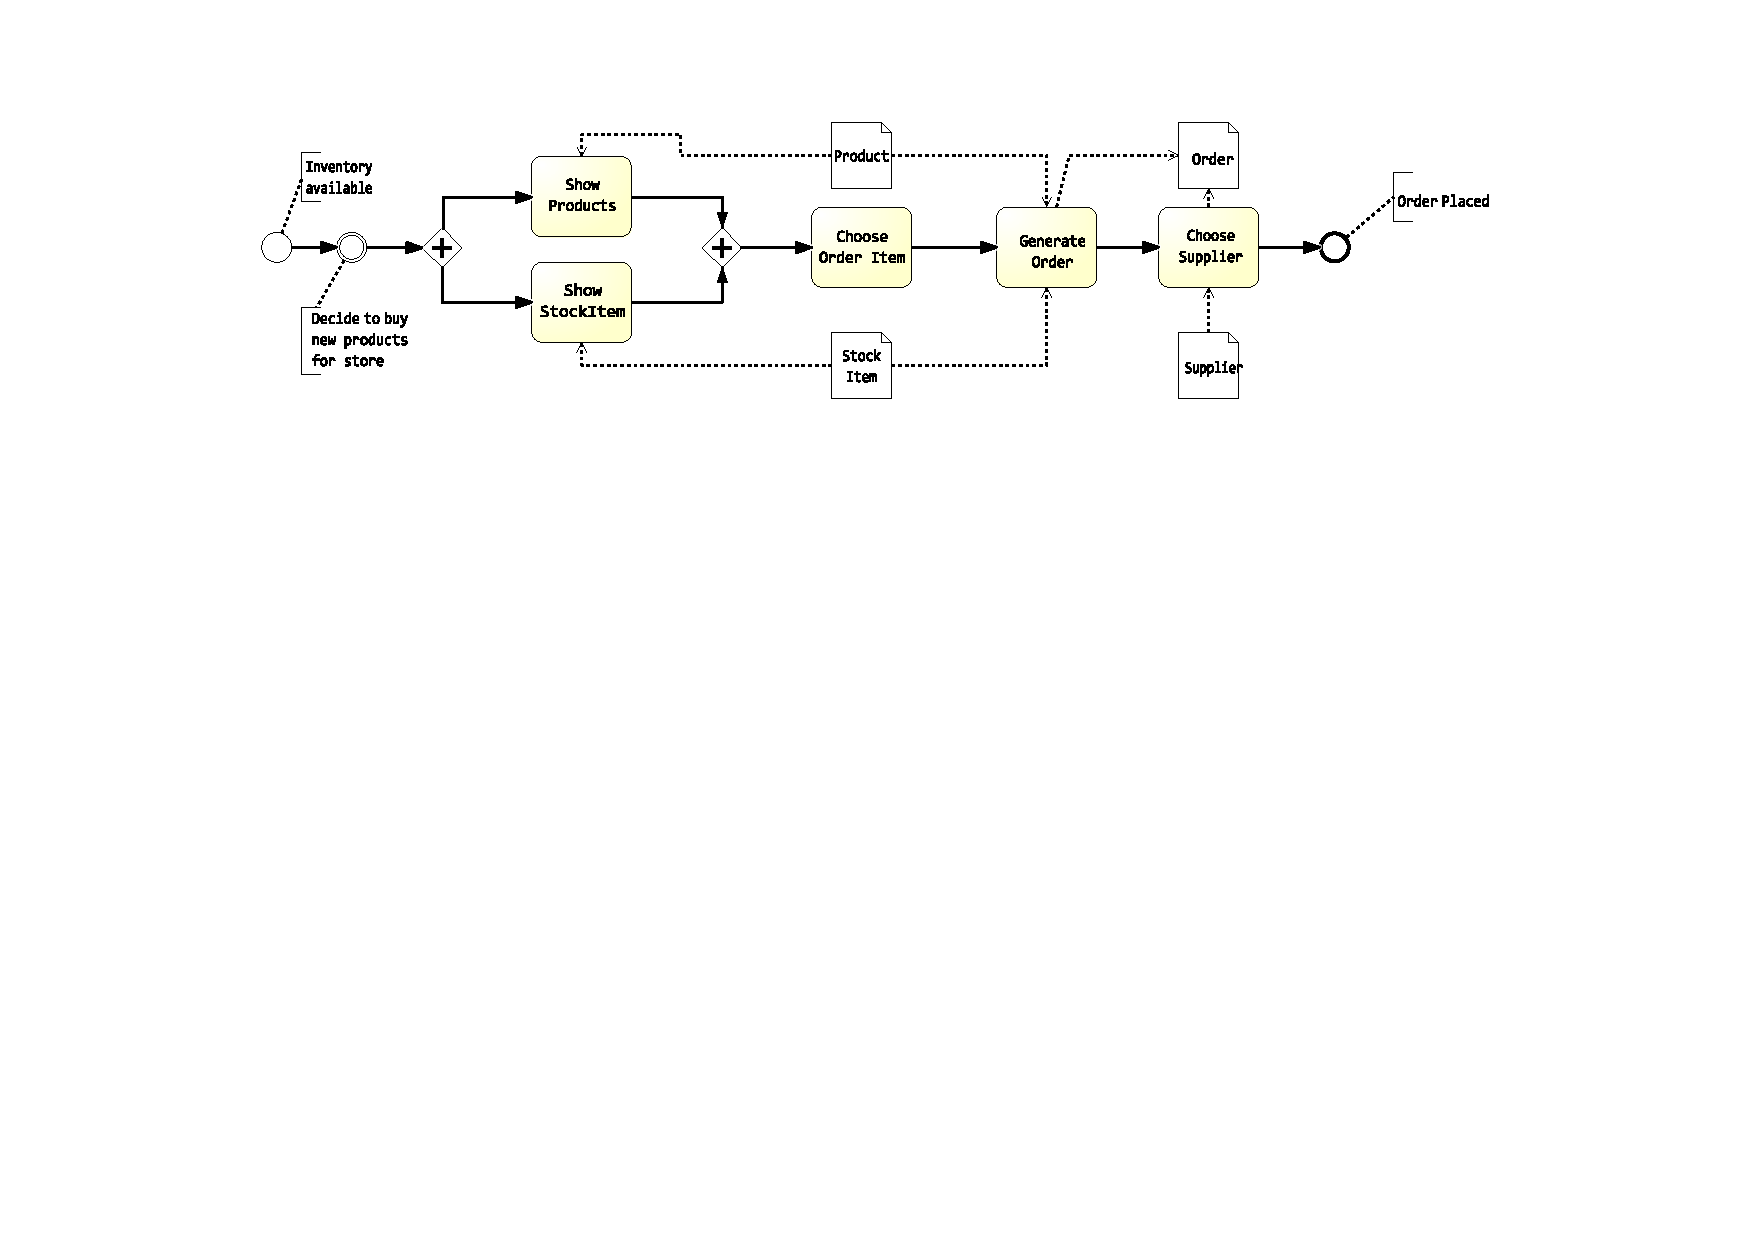
\includegraphics[width=\textwidth, trim={6cm 14cm 6cm 1cm}]{img/UC3.pdf}
	\caption{UC3 - Order Products}
	\label{fig:UC3}
\end{figure}


%"l, b, r, t"
\begin{figure}[h!]
	\centering
	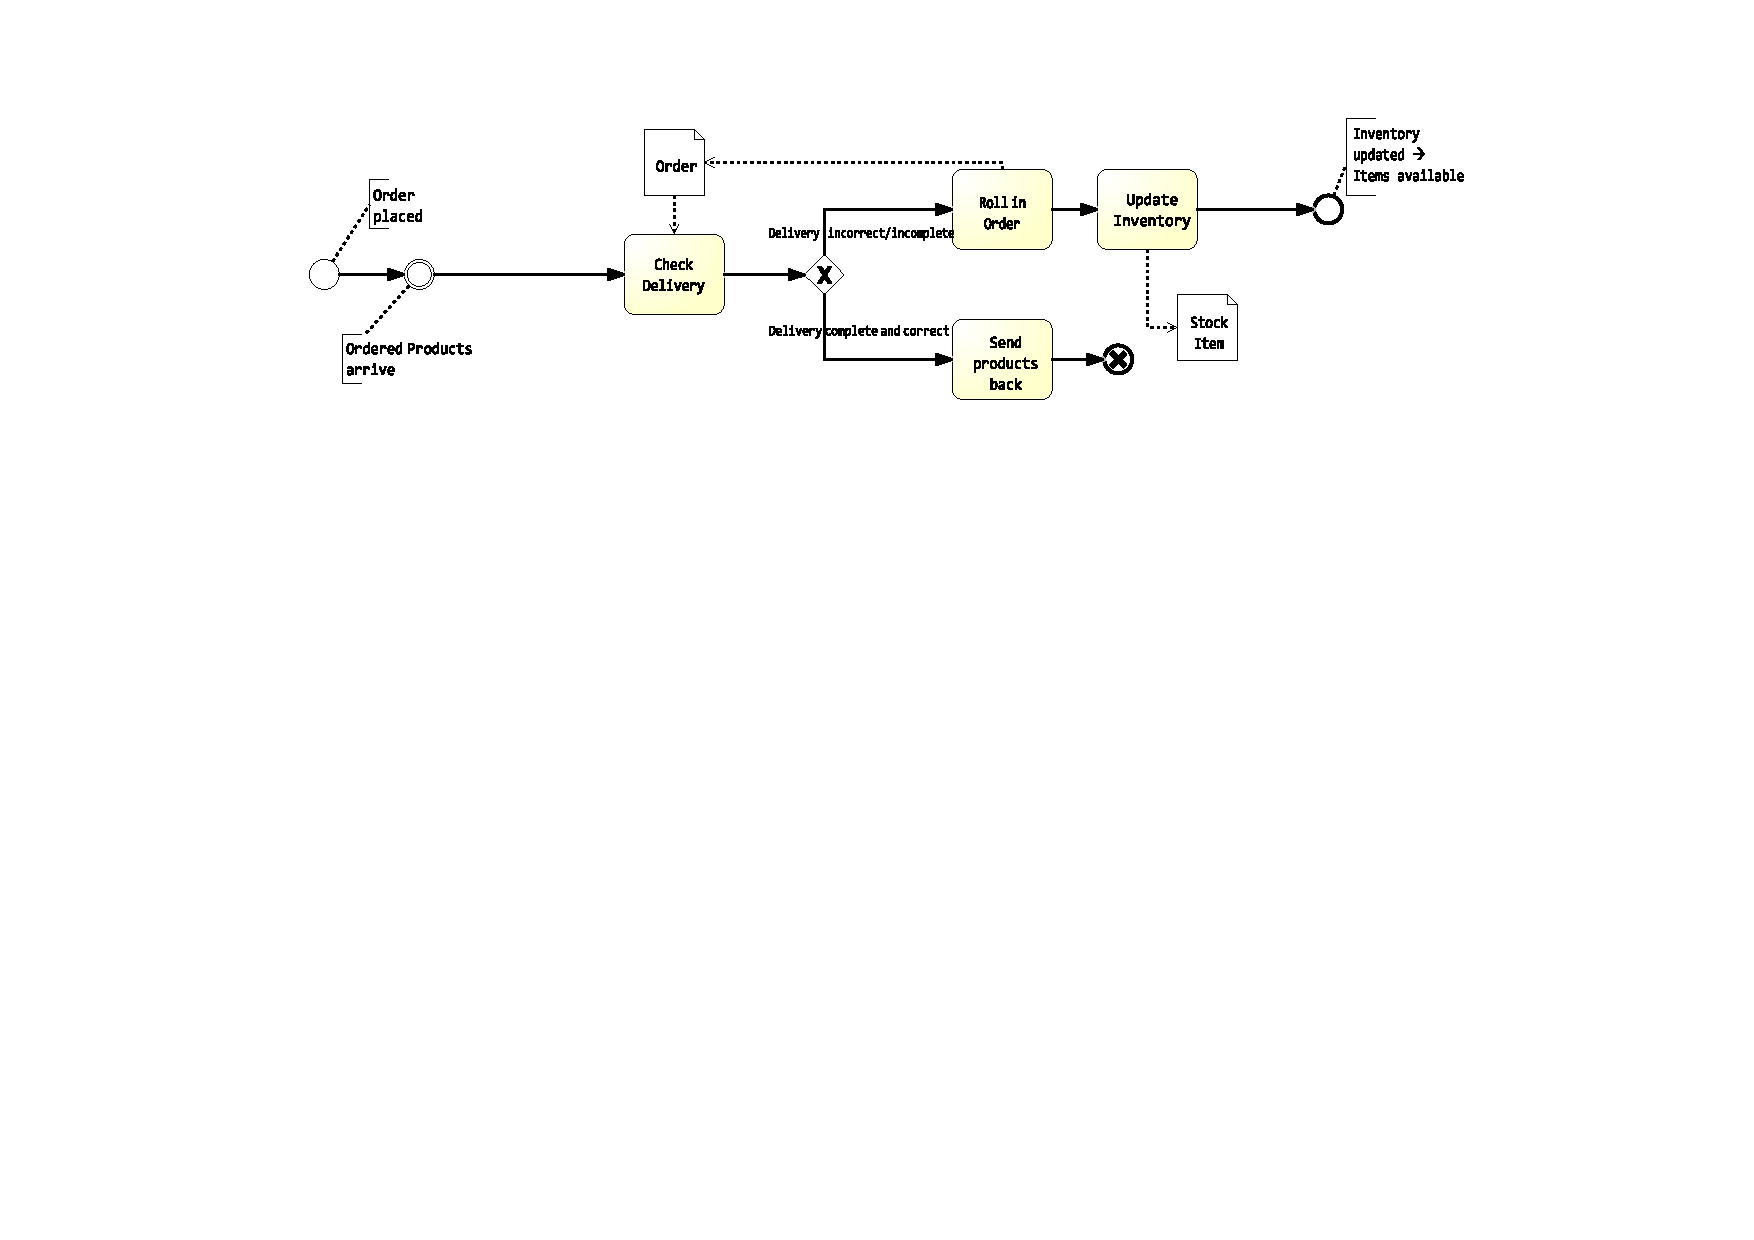
\includegraphics[width=\textwidth, trim={6.5cm 14cm 6cm 1cm}]{img/UC4.pdf}
	\caption{UC4 - Receive Ordered Products }
	\label{fig:UC4}
\end{figure}

\pagebreak

%"l, b, r, t"
\begin{figure}[h!]
	\centering
	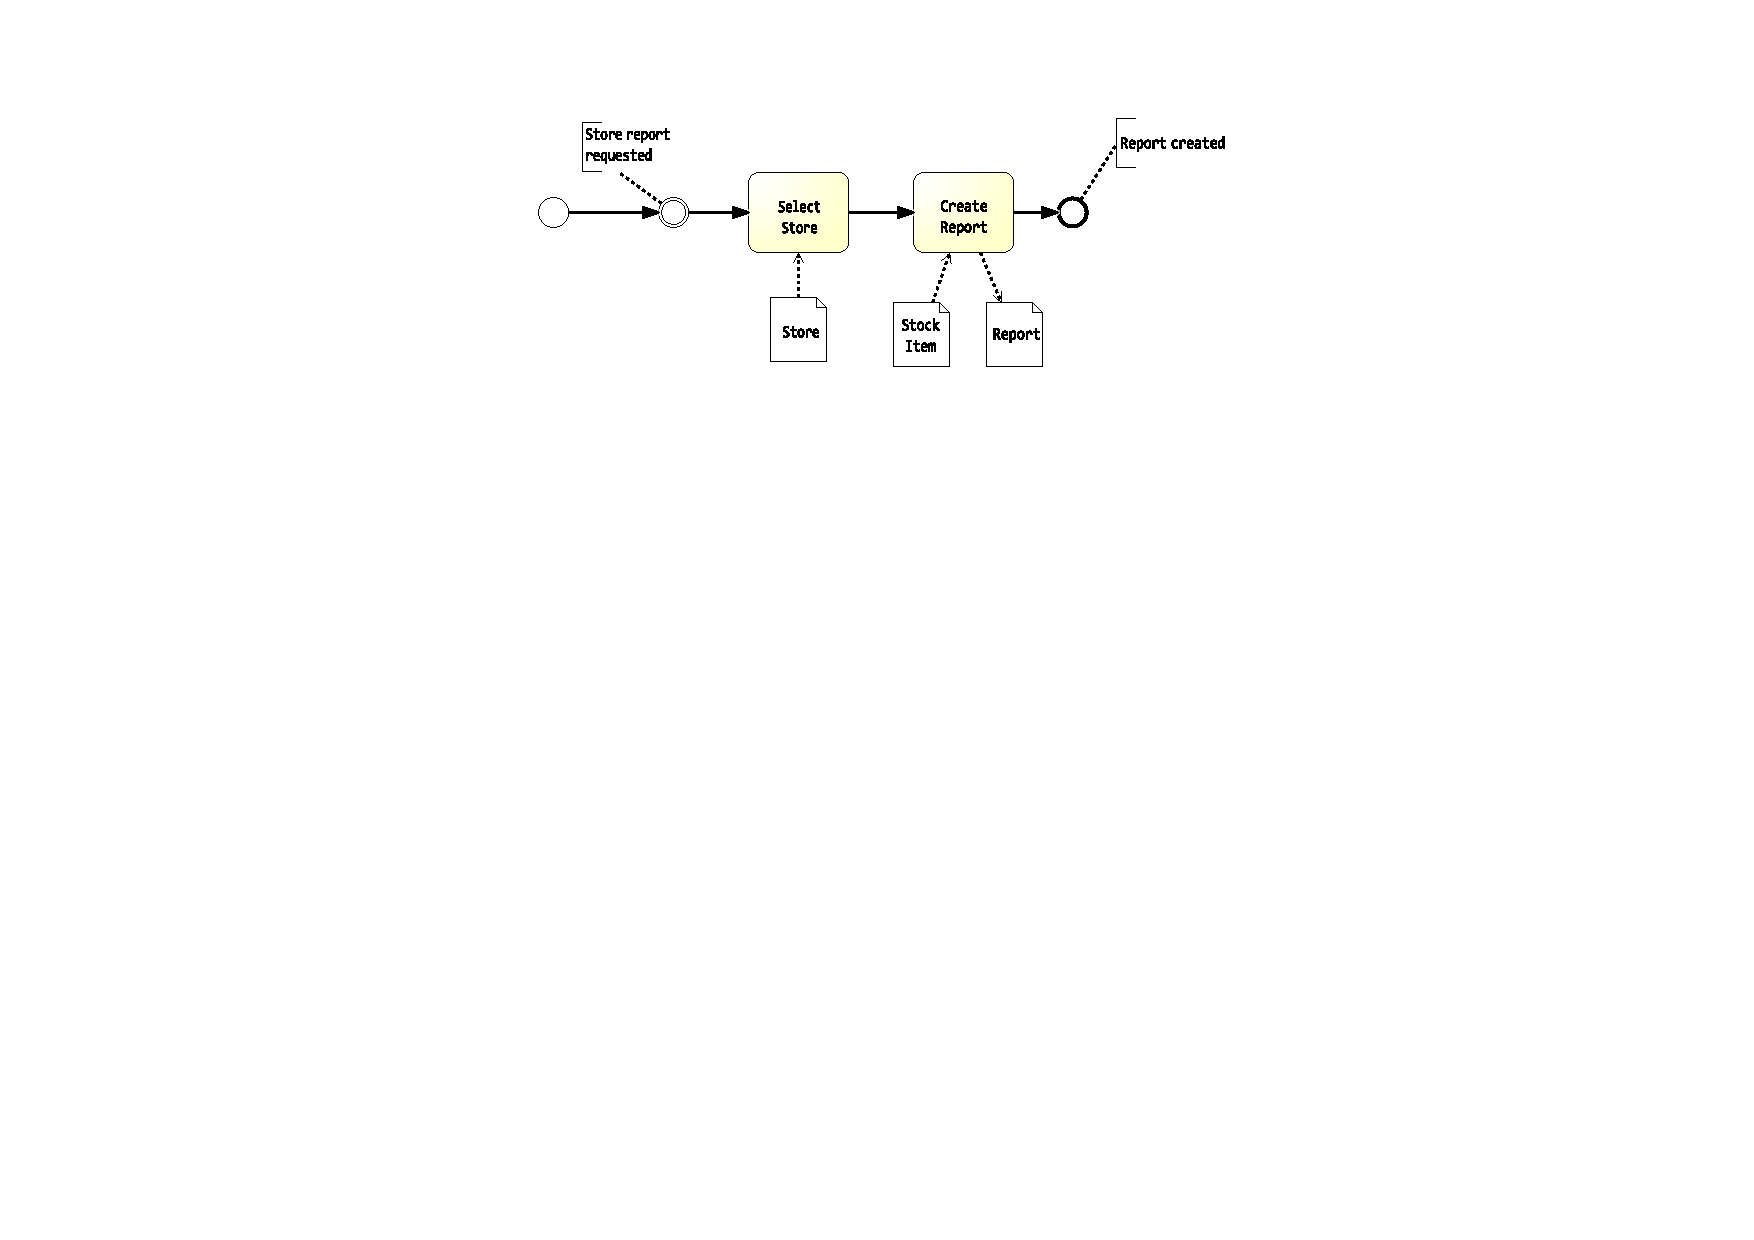
\includegraphics[width=\textwidth, trim={6cm 15cm 7cm 1cm}]{img/UC5.pdf}
	\caption{UC5 - Show Stock Reports }
	\label{fig:UC5}
\end{figure}

%"l, b, r, t"
\begin{figure}[h!]
	\centering
	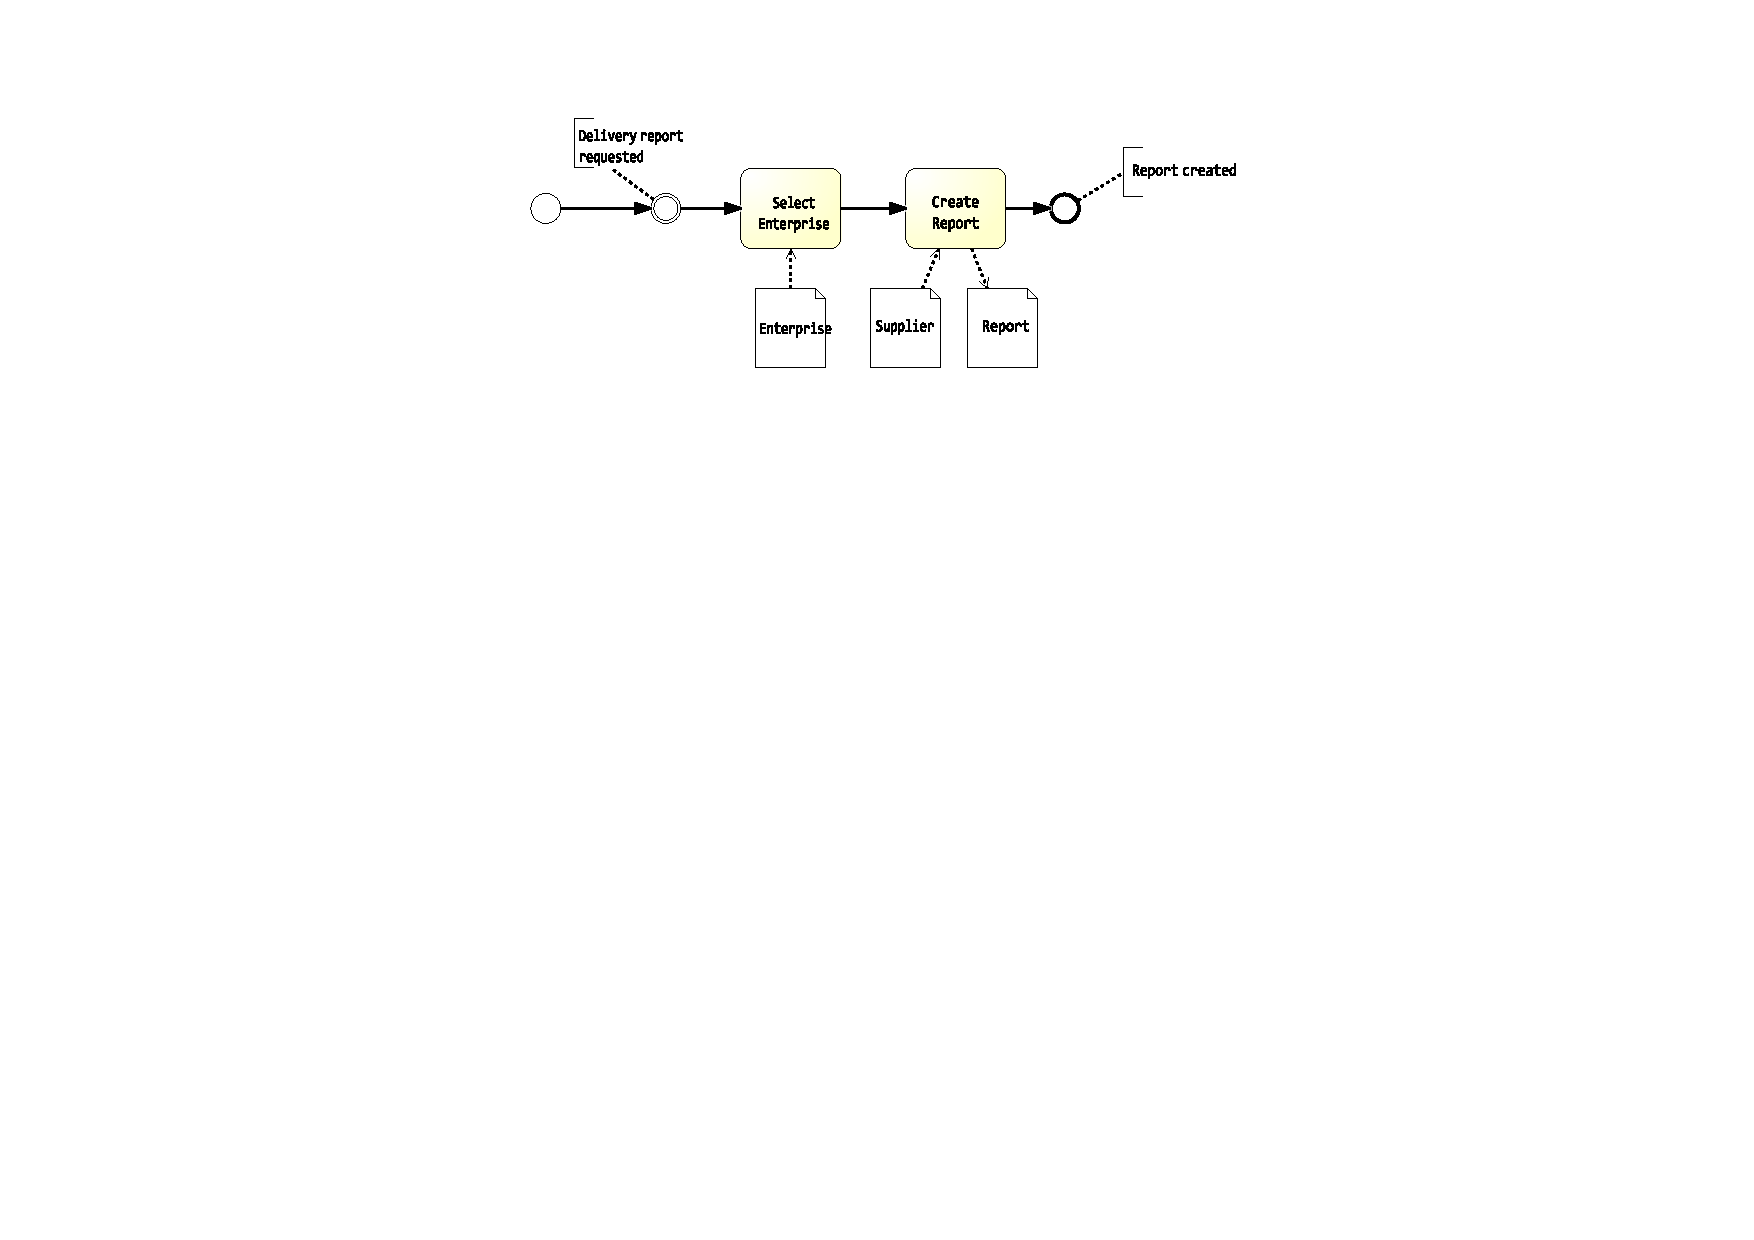
\includegraphics[width=\textwidth, trim={6cm 14.5cm 7cm 1cm}]{img/UC6.pdf}
	\caption{UC6 - Show Delivery Reports }
	\label{fig:UC6}
\end{figure}

%"l, b, r, t"
\begin{figure}[h!]
	\centering
	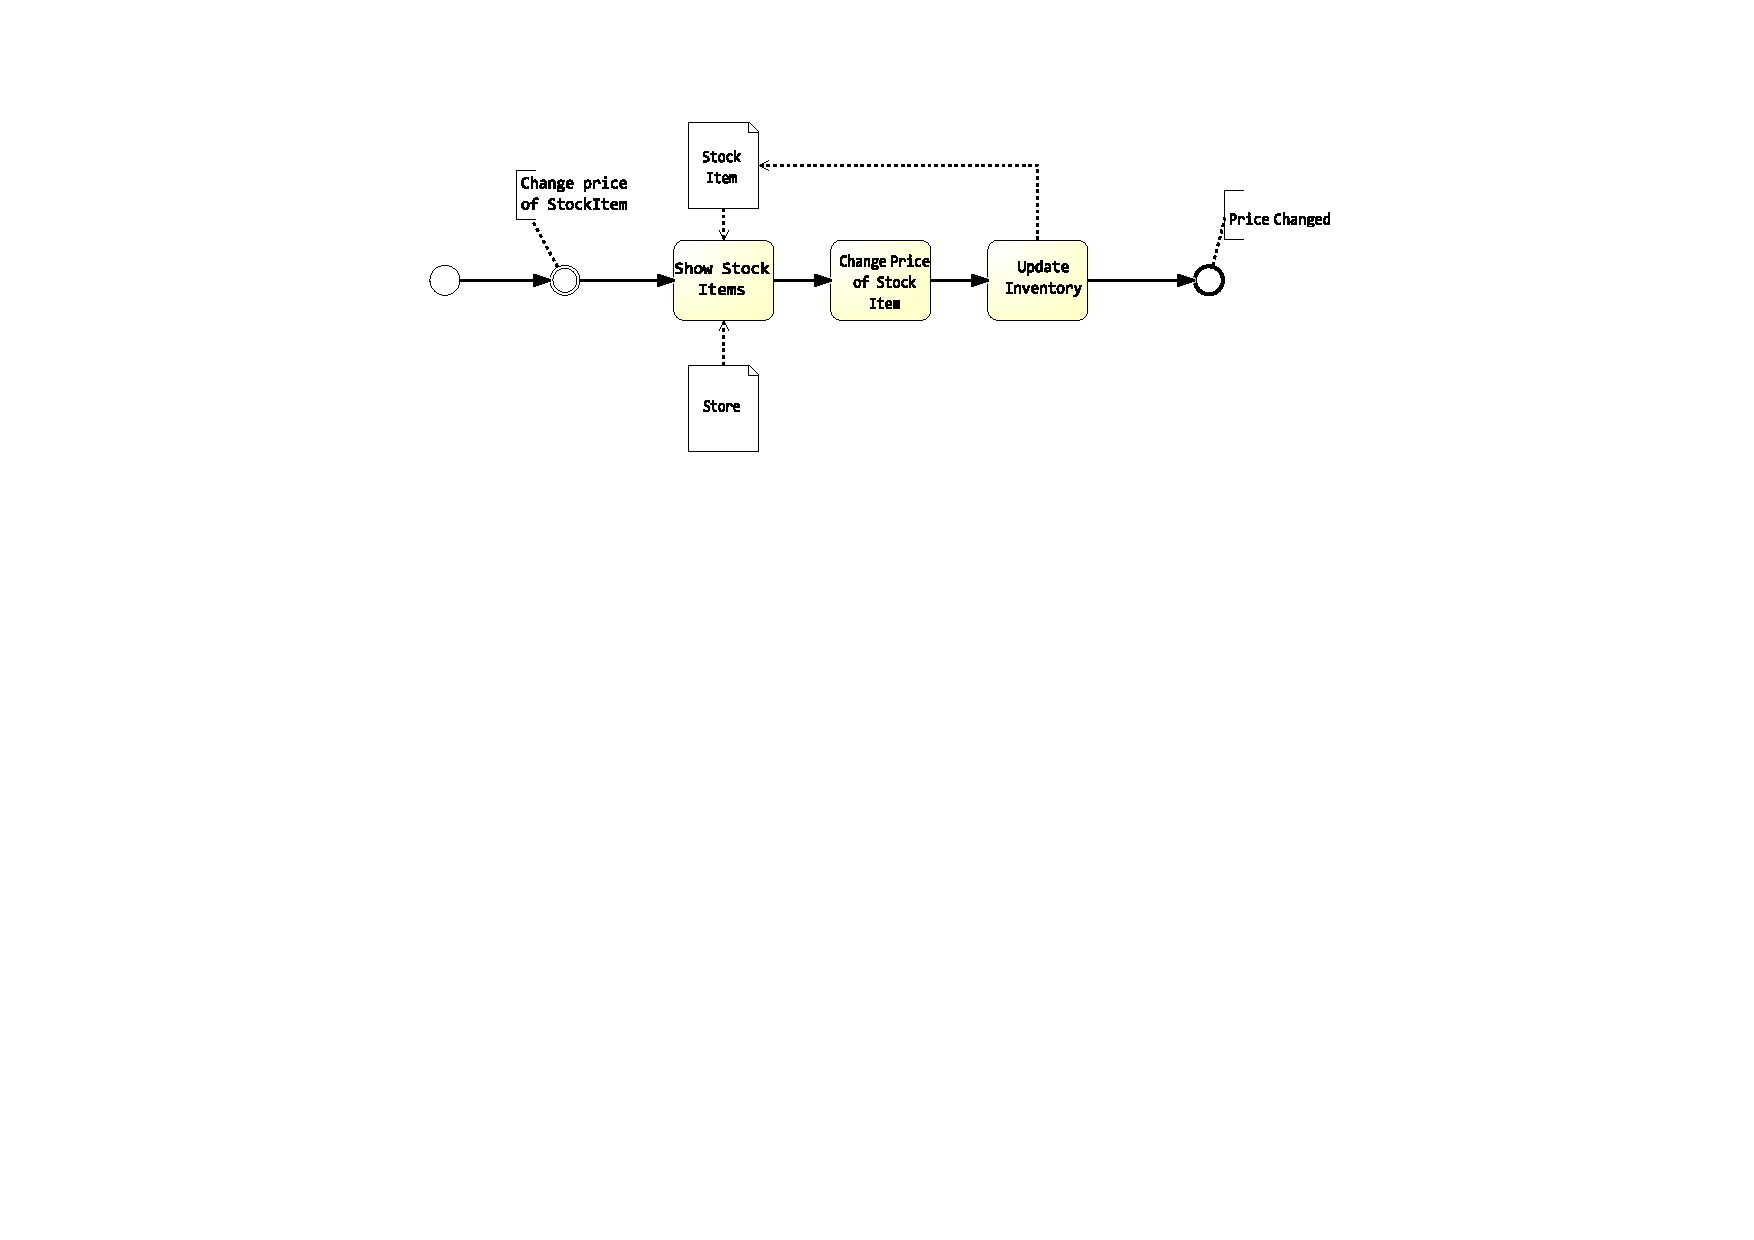
\includegraphics[width=\textwidth, trim={6cm 13cm 7cm 1cm}]{img/UC7.pdf}
	\caption{UC7 - Change Price }
	\label{fig:UC7}
\end{figure}

\clearpage

\section{Control Flow Diagrams}
\label{sec:appendix:ControlFlow}

%"l, b, r, t"
\begin{figure}[h!]
	\centering
	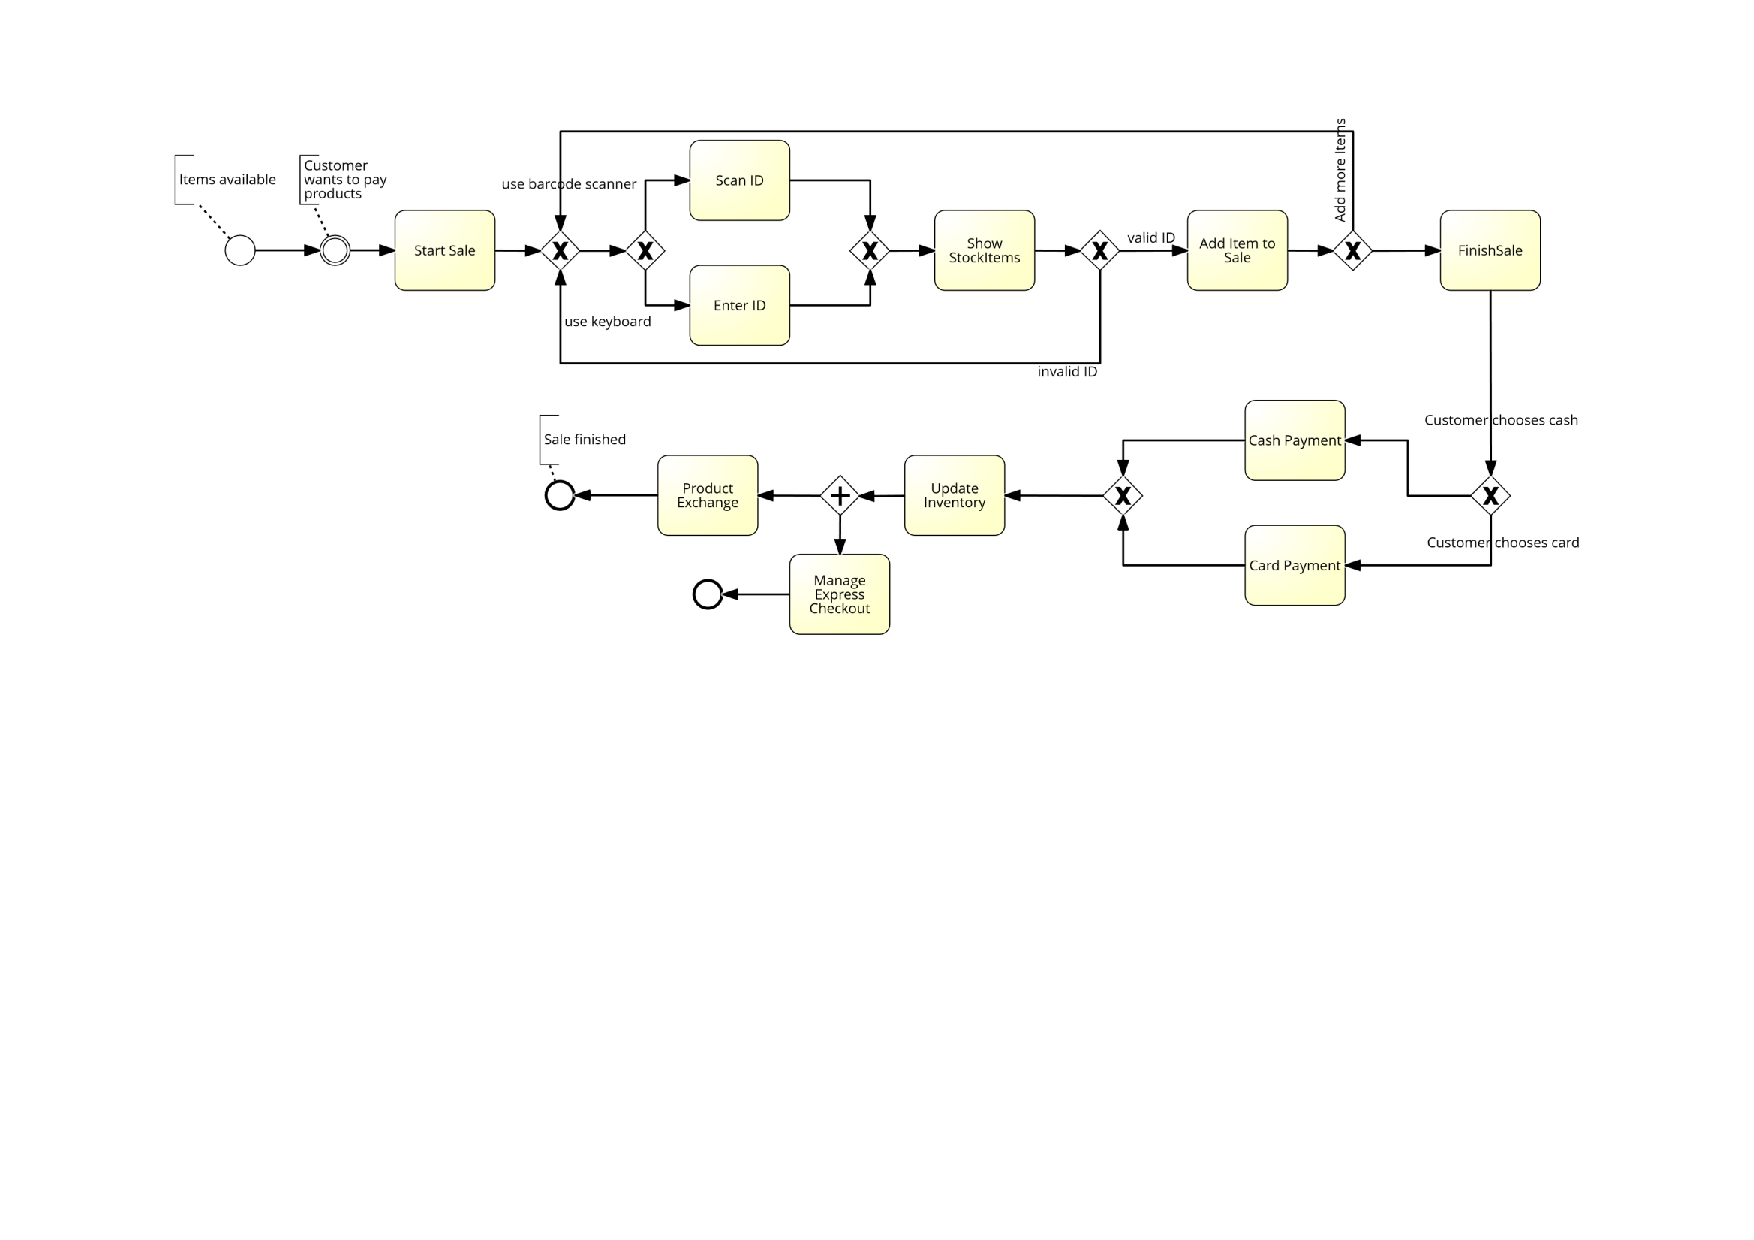
\includegraphics[width=\textwidth, trim={5cm 10cm 4cm 1cm}]{img/UC1Control.pdf}
	\caption{Control Flow UC1 - Start Sale}
	\label{fig:UC1Control}
\end{figure}


%"l, b, r, t"
\begin{figure}[h!]
	\centering
	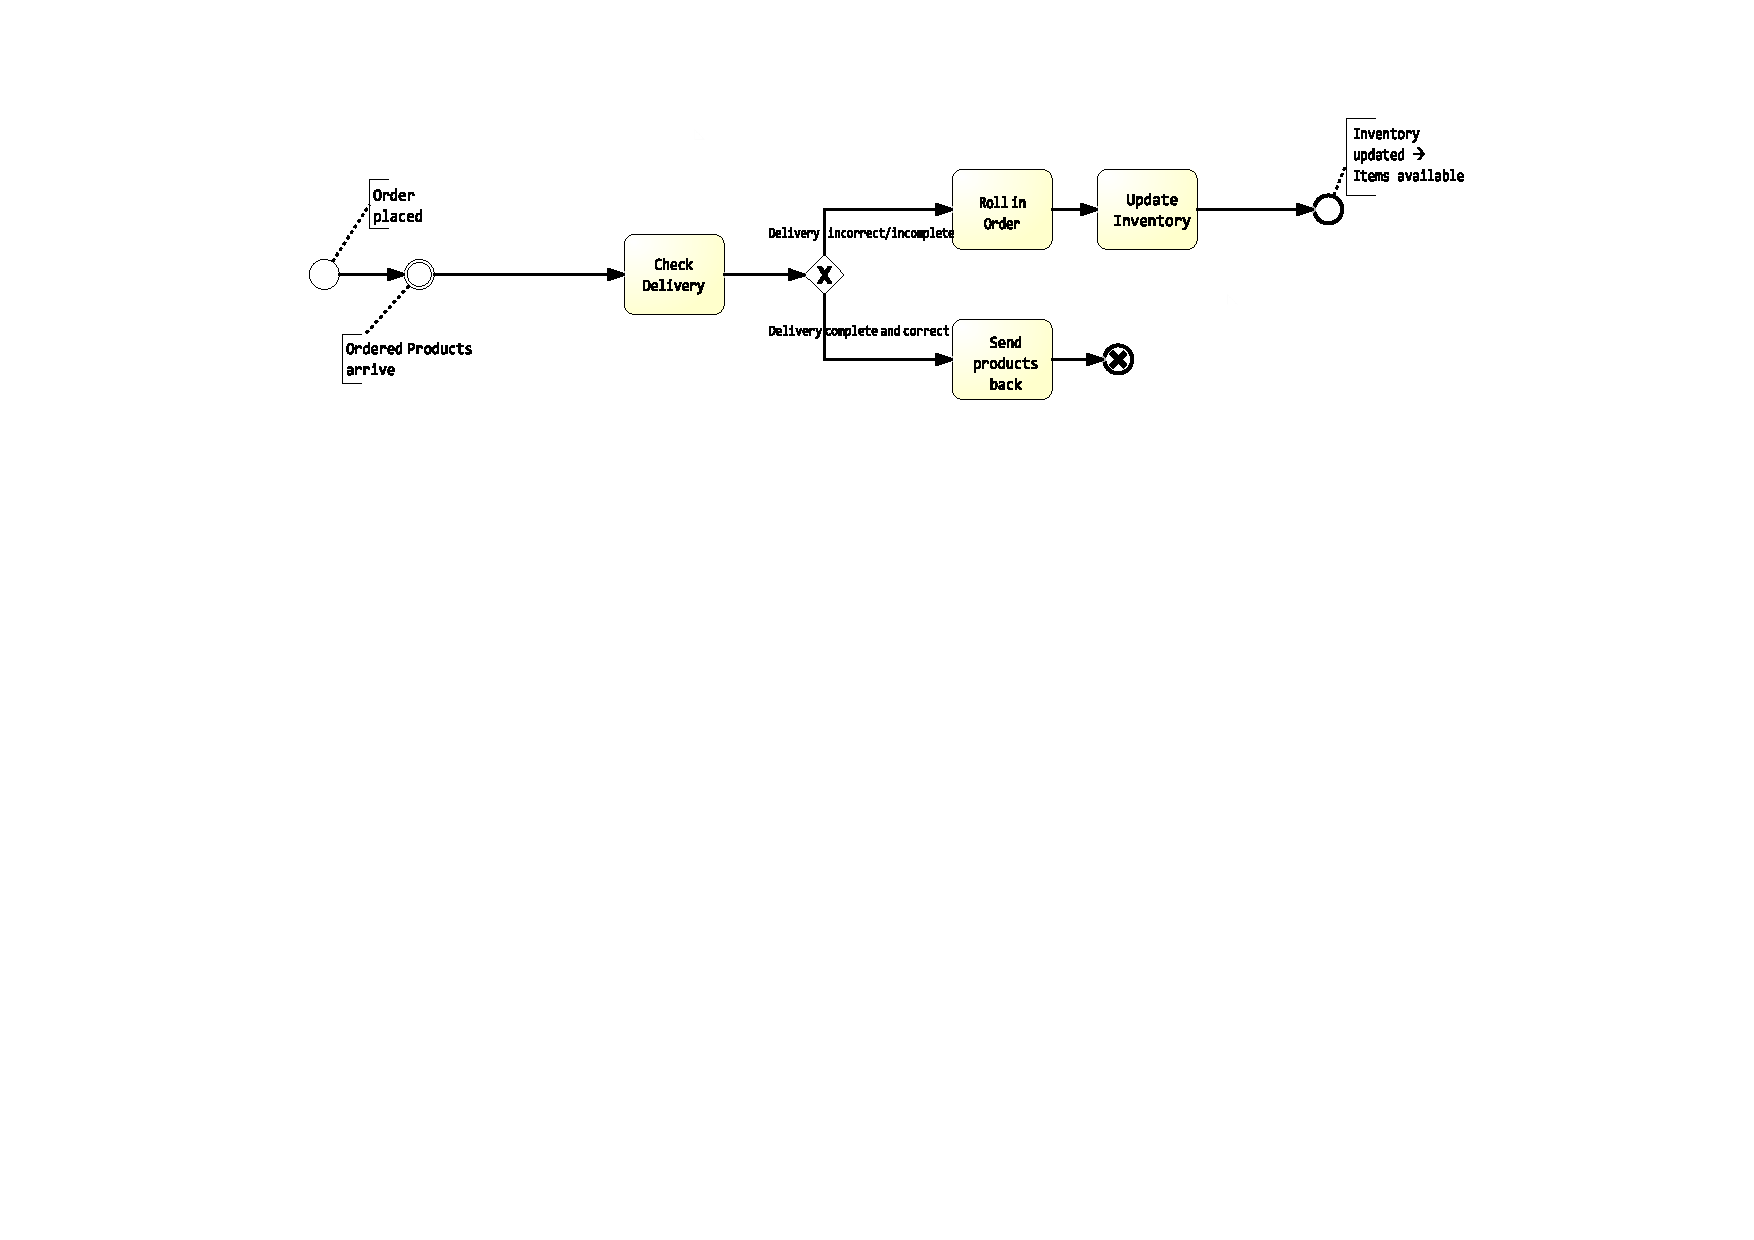
\includegraphics[width=\textwidth, trim={7cm 14cm 6cm 1cm}]{img/UC4Control.pdf}
	\caption{Control Flow UC4 - Receive Ordered Products }
	\label{fig:UC4Control}
\end{figure}

\pagebreak

%"l, b, r, t"
\begin{figure}[h!]
	\centering
	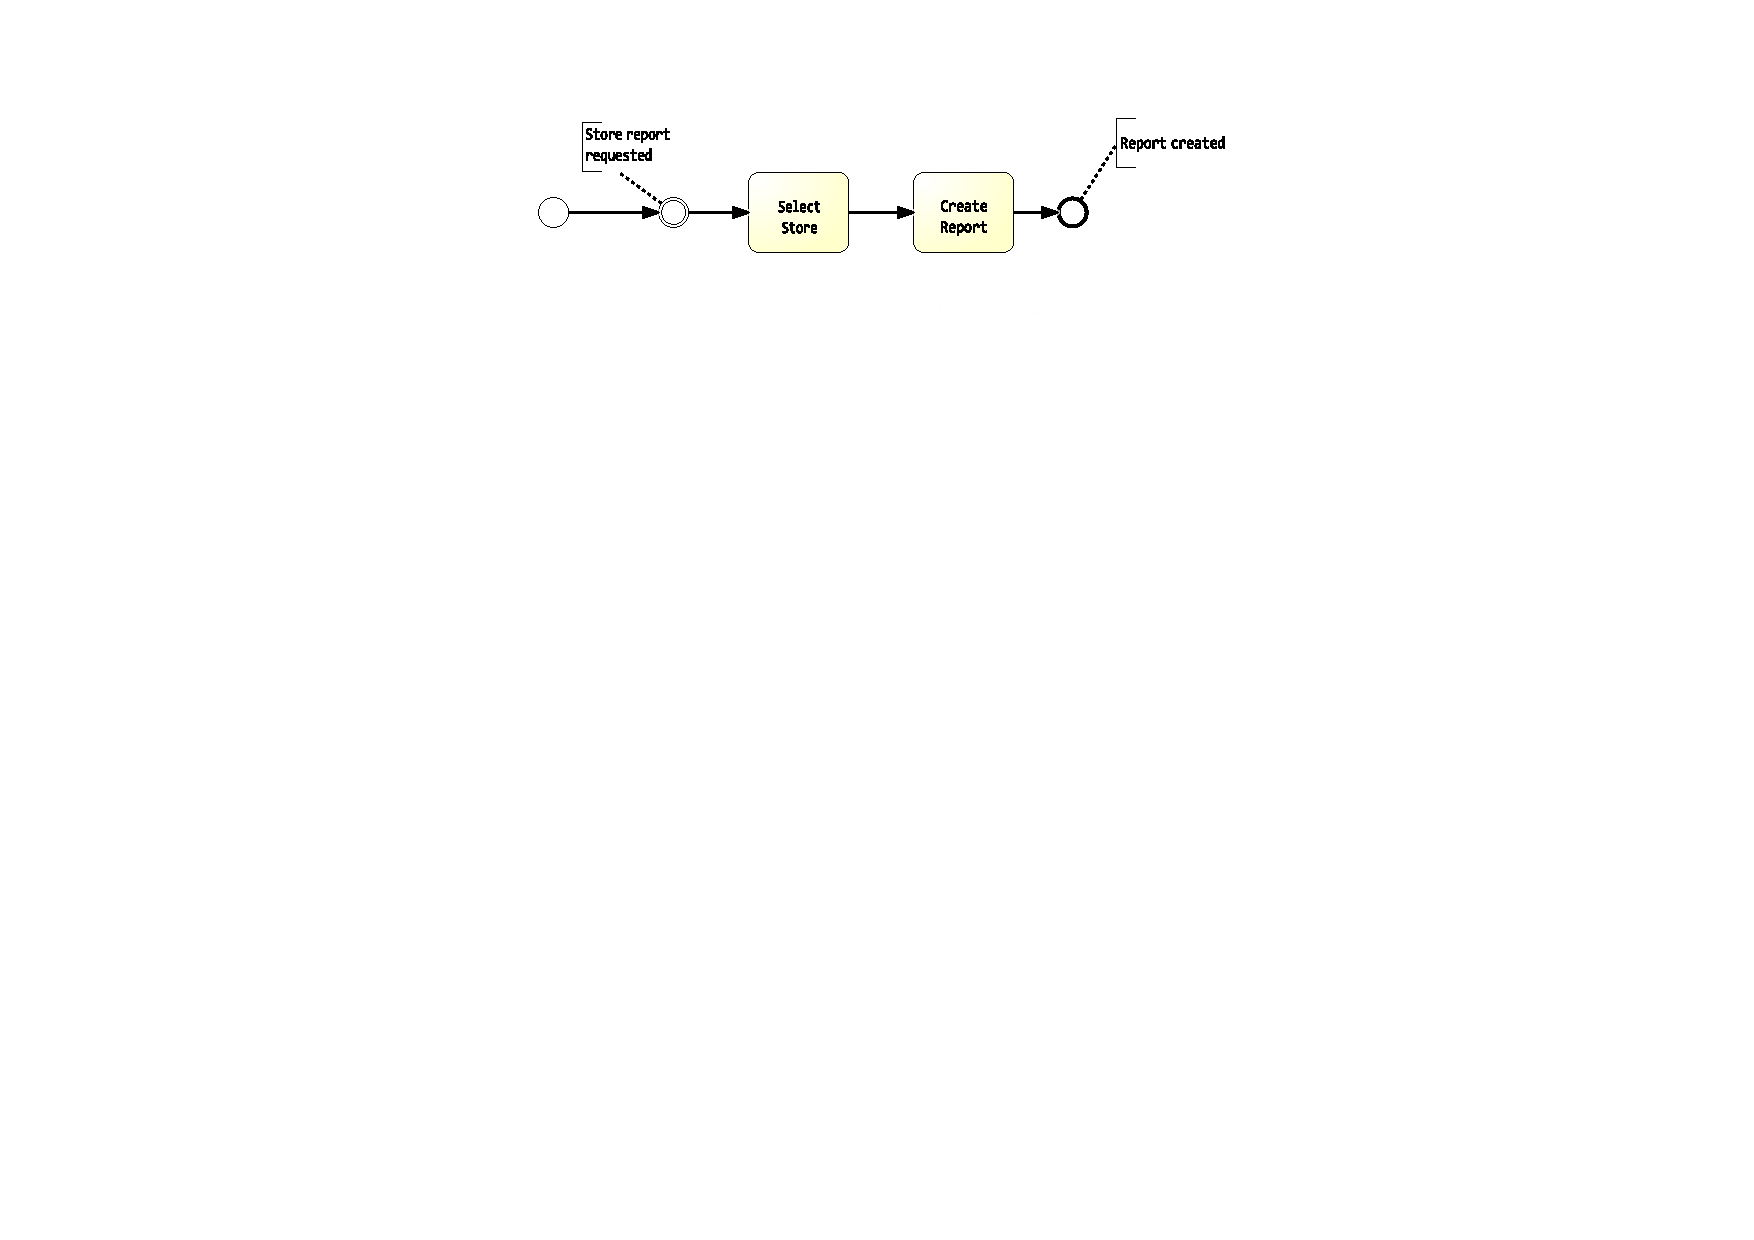
\includegraphics[width=\textwidth, trim={6cm 16.5cm 7cm 1cm}]{img/UC5Control.pdf}
	\caption{Control Flow UC5 - Show Stock Reports }
	\label{fig:UC5Control}
\end{figure}

%"l, b, r, t"
\begin{figure}[h!]
	\centering
	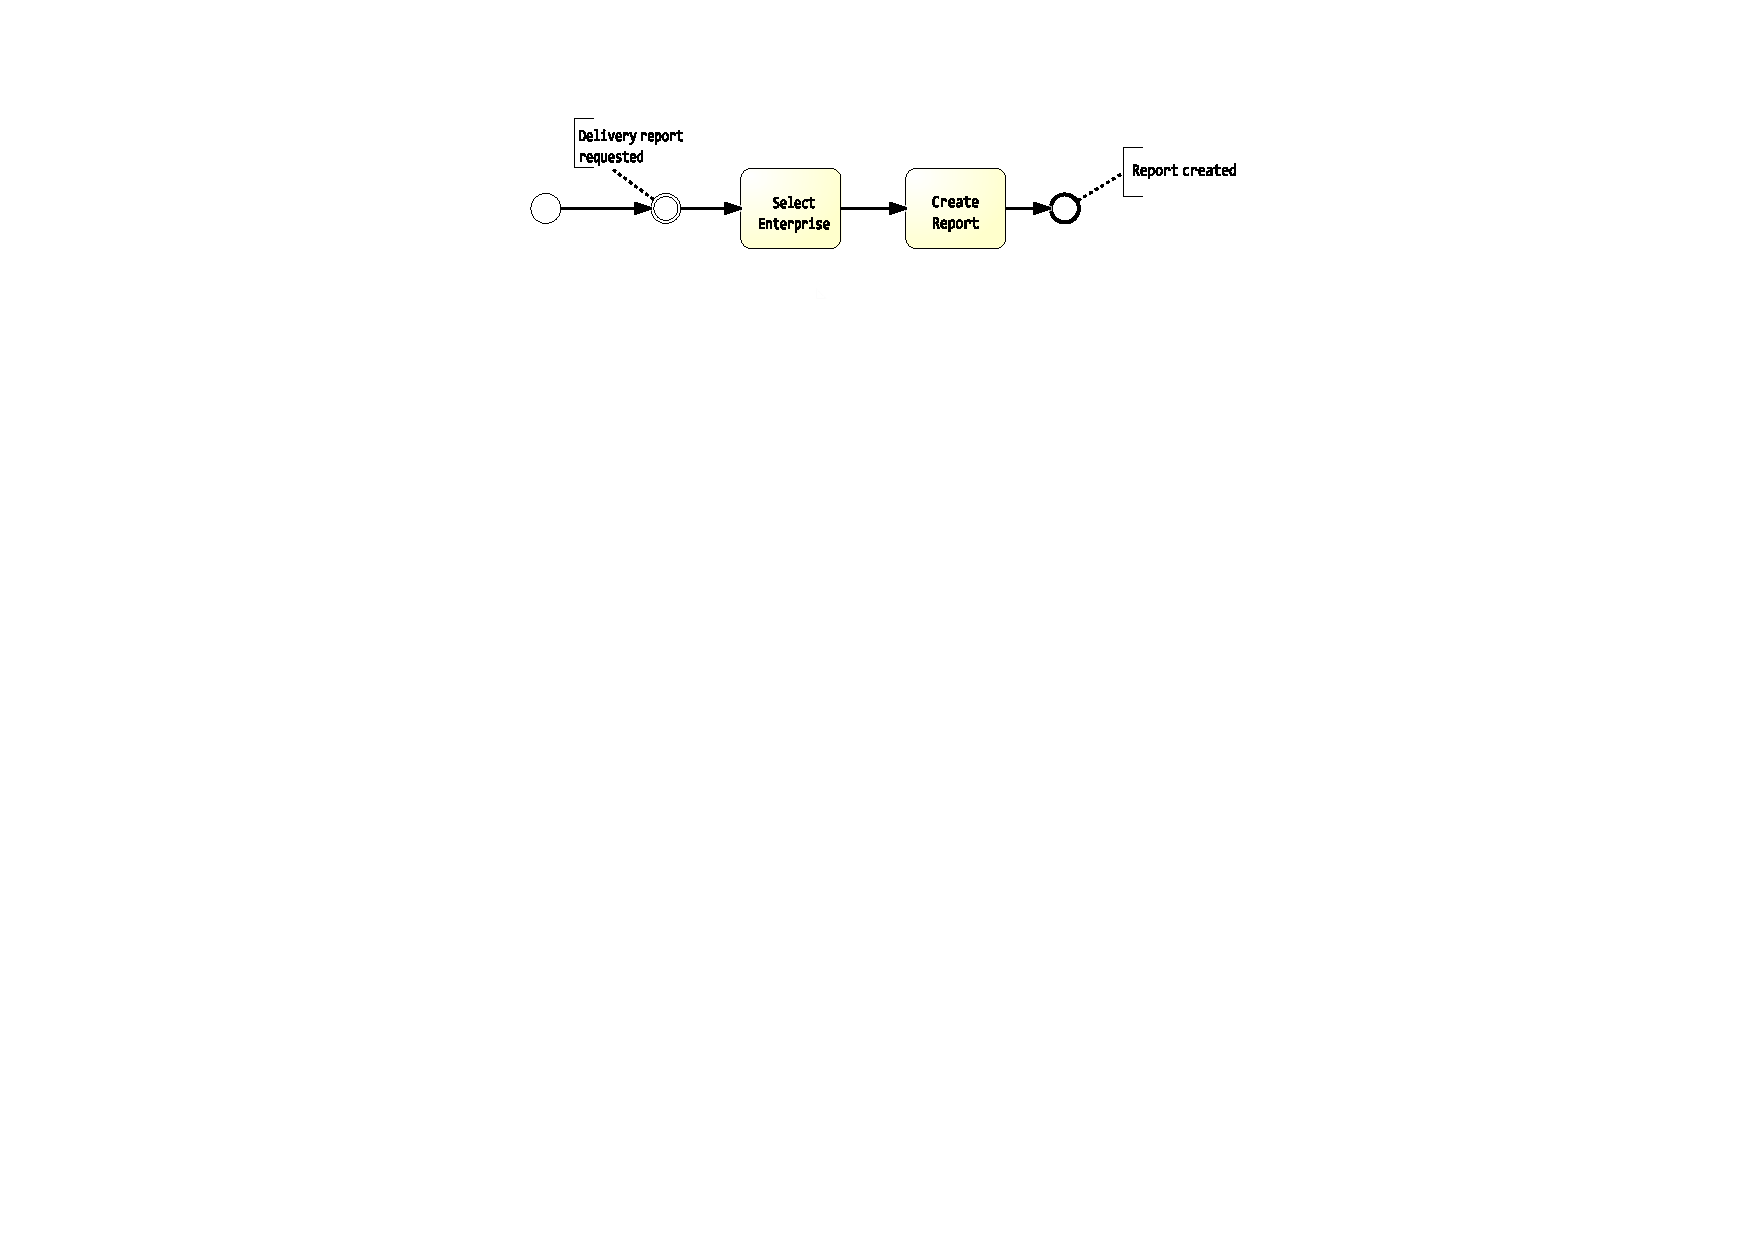
\includegraphics[width=\textwidth, trim={6cm 16.5cm 7cm 1cm}]{img/UC6Control.pdf}
	\caption{Control Flow UC6 - Show Delivery Reports }
	\label{fig:UC6Control}
\end{figure}

%"l, b, r, t"
\begin{figure}[h!]
	\centering
	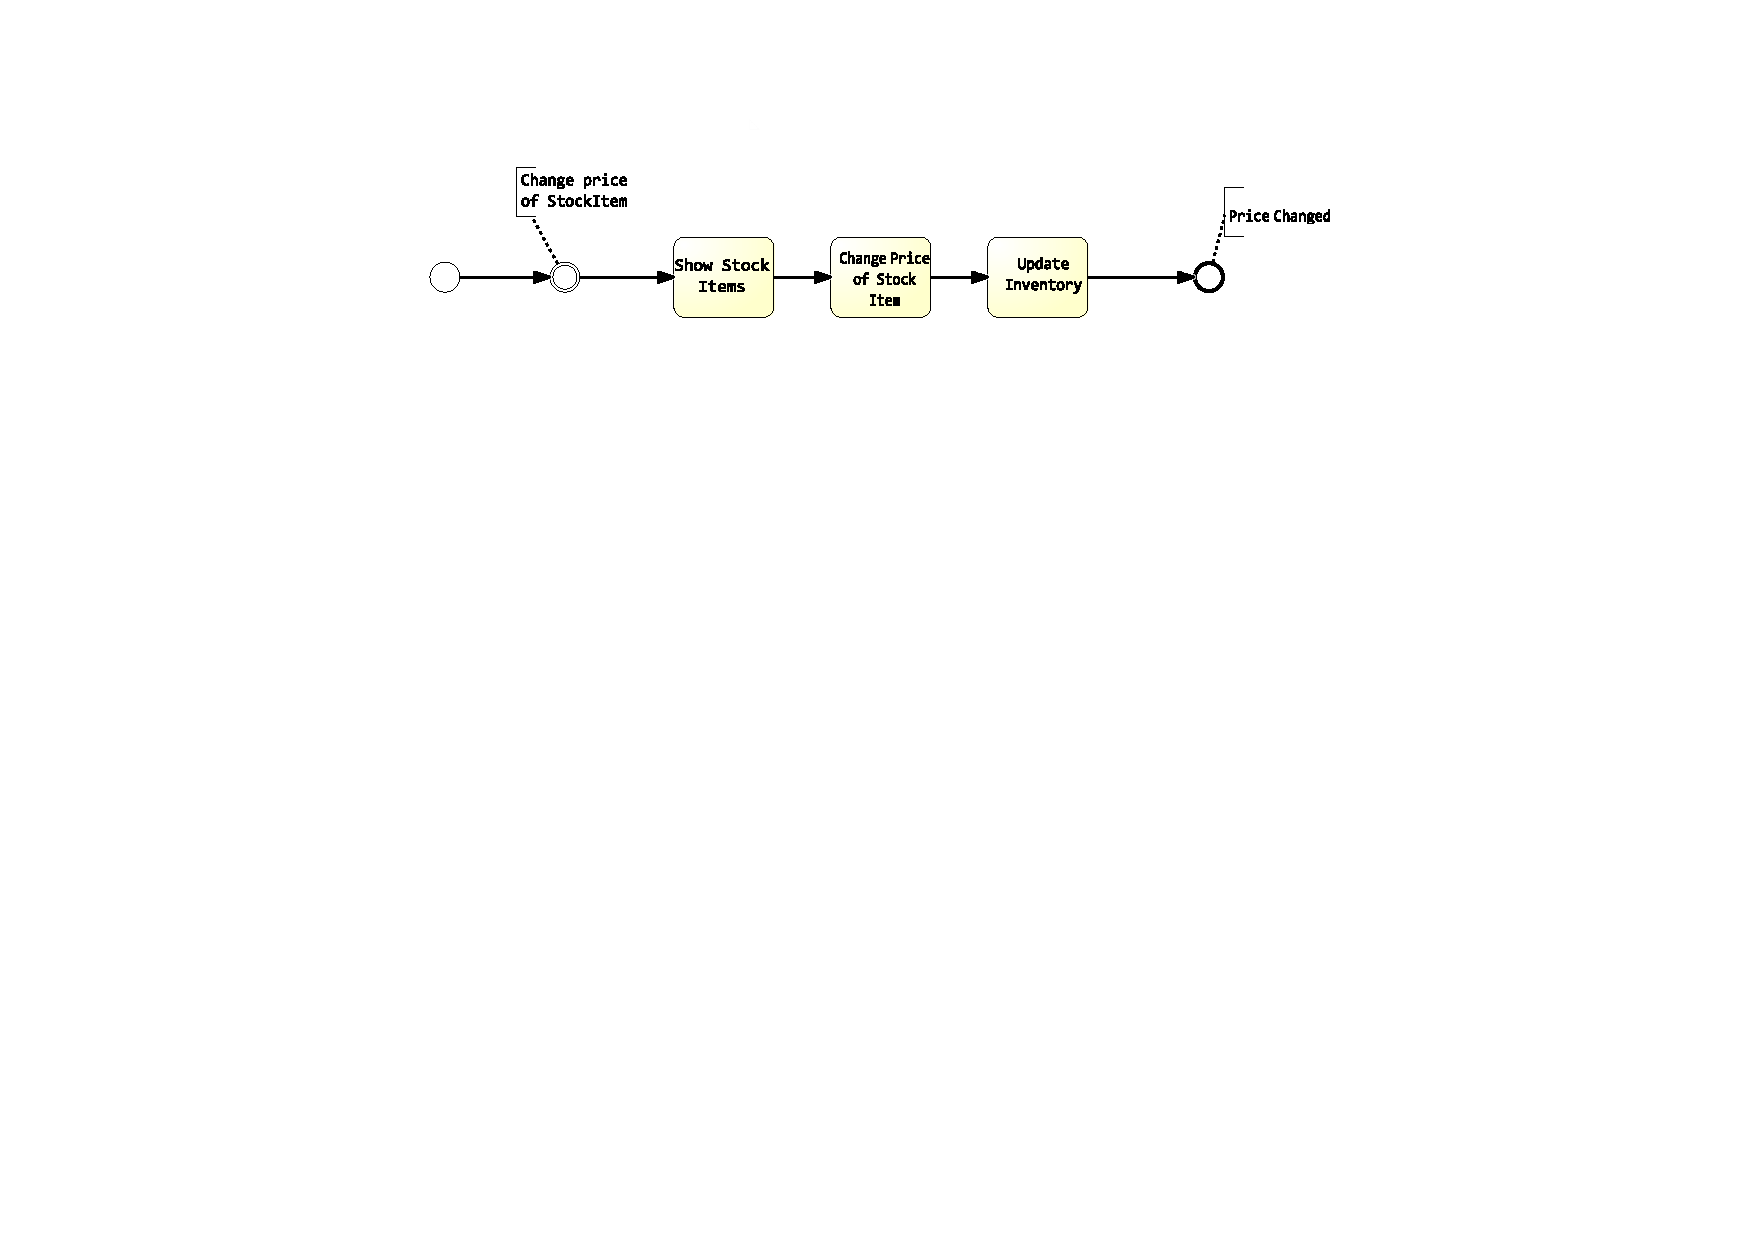
\includegraphics[width=\textwidth, trim={6cm 15.5cm 7cm 1cm}]{img/UC7Control.pdf}
	\caption{Control Flow UC7 - Change Price }
	\label{fig:UC7Control}
\end{figure}


\pagebreak












\section{Data Flow Diagrams}
\label{sec:appendix:DataFlow}

%"l, b, r, t"
\begin{figure}[h!]
	\centering
	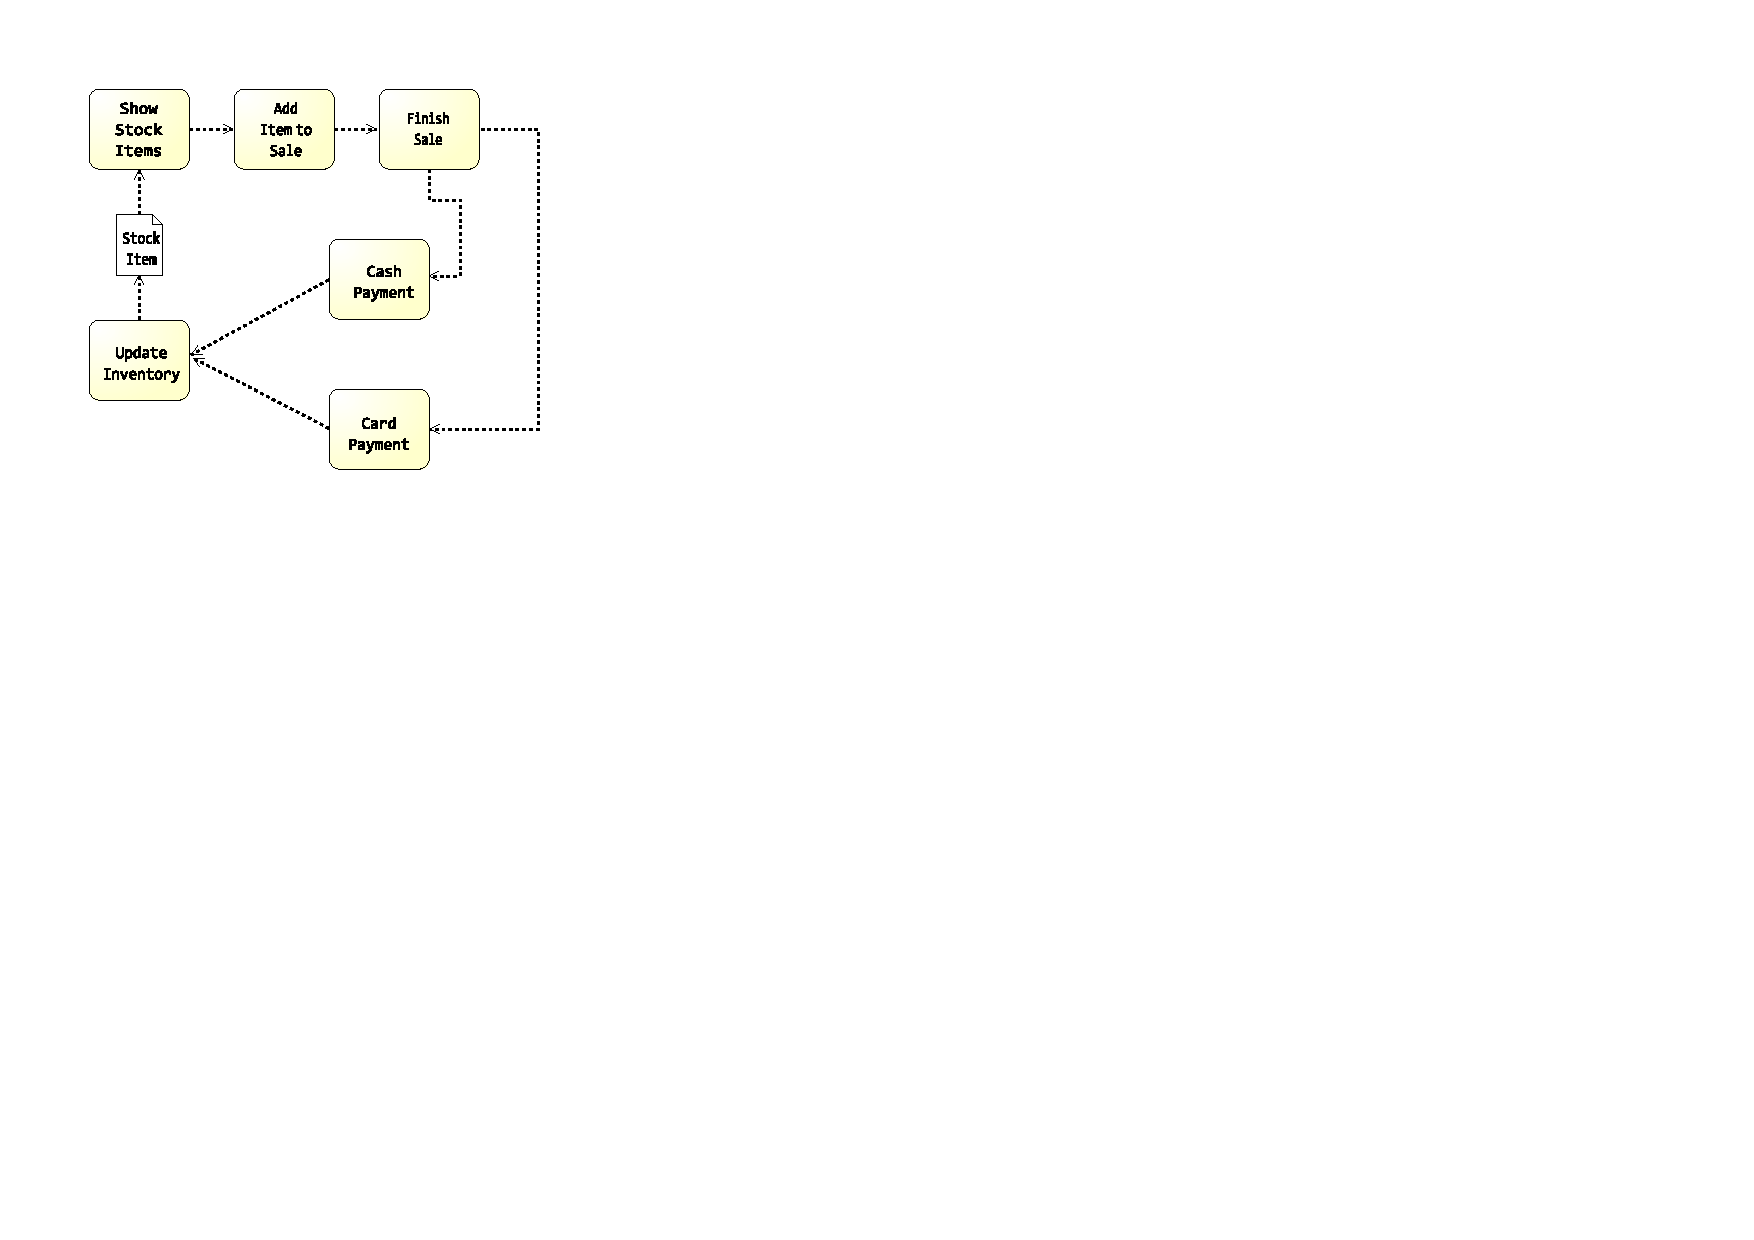
\includegraphics[width=5.5cm, trim={3cm 13cm 22cm 1cm}]{img/UC1DFD.pdf}
	\caption{Data Flow UC1 - Start Sale}
	\label{fig:UC1DFD}
\end{figure}


%"l, b, r, t"
\begin{figure}[h!]
	\centering
	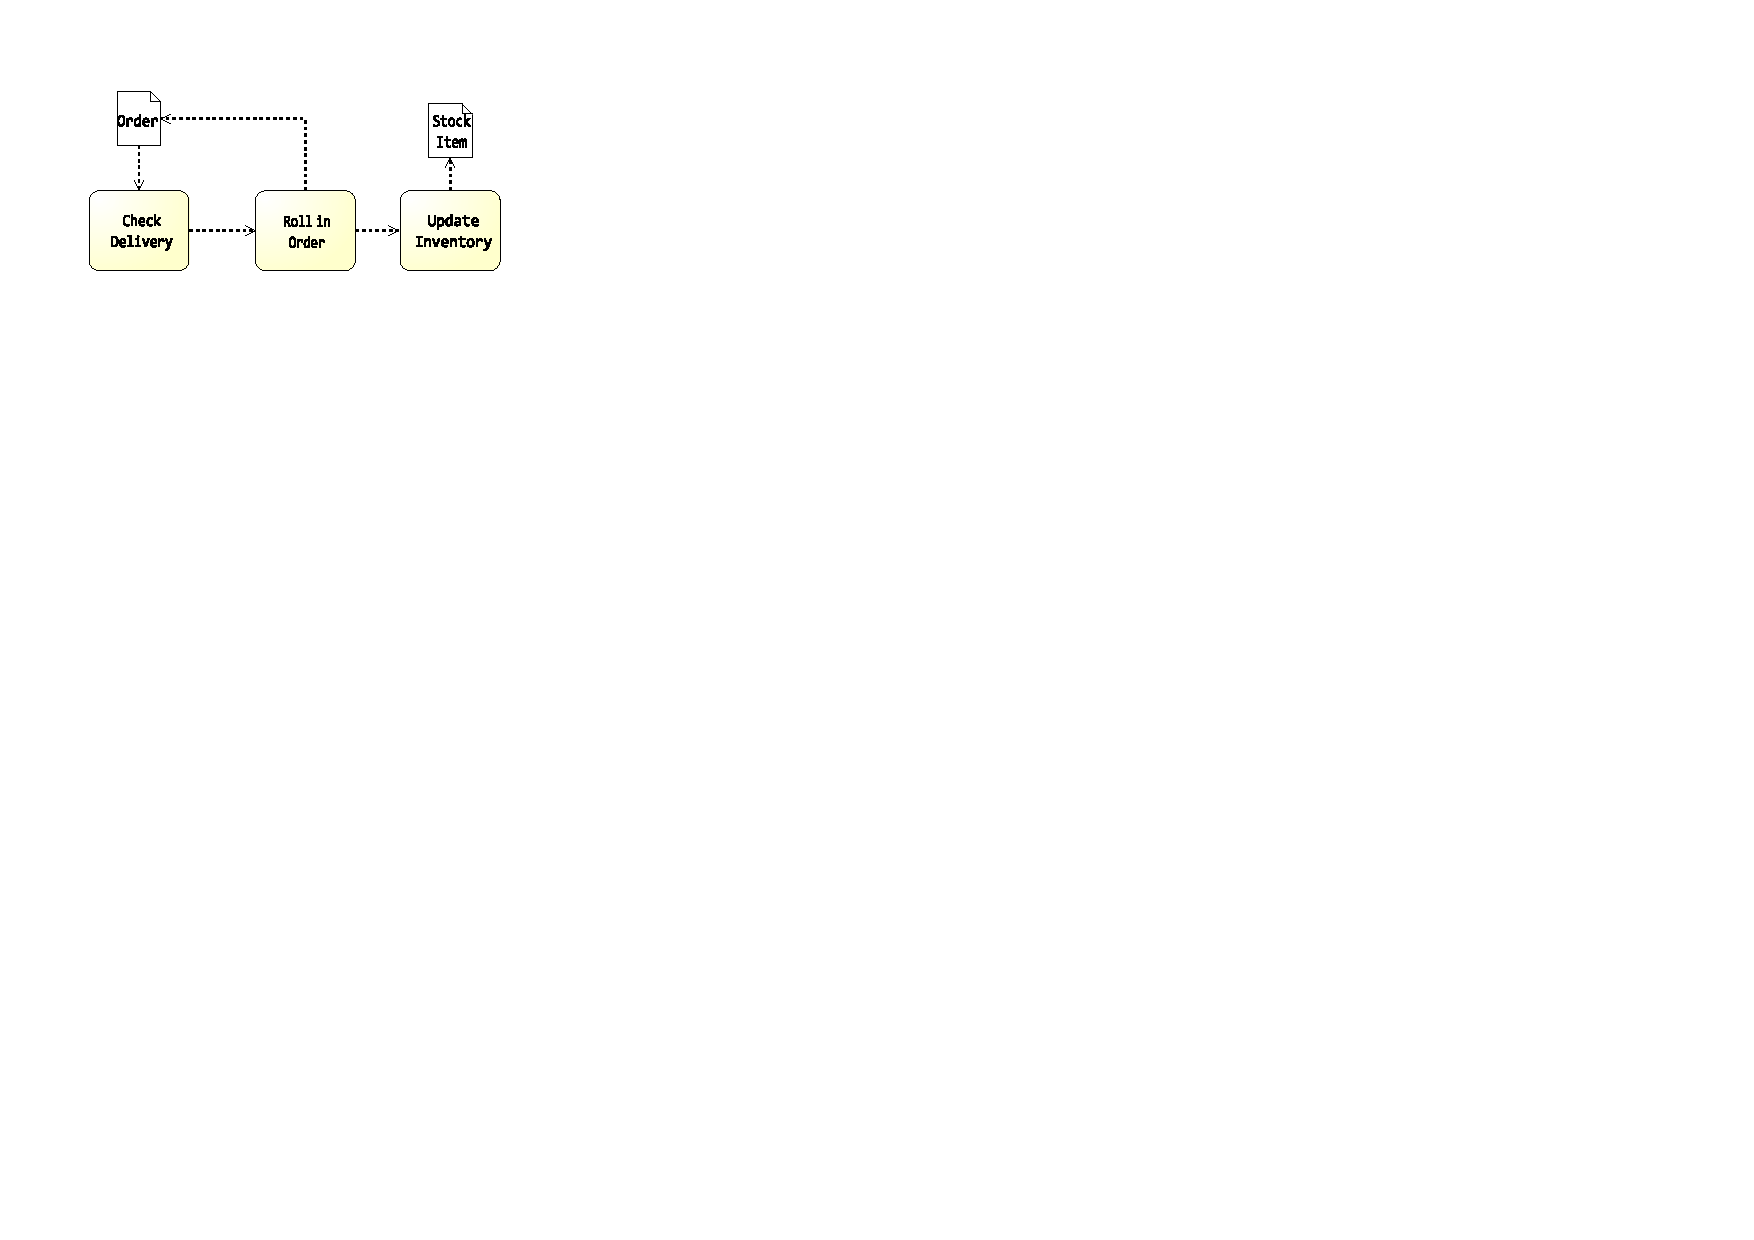
\includegraphics[width=5.5cm, trim={3cm 16cm 22cm 1cm}]{img/UC4DFD.pdf}
	\caption{Data Flow UC4 - Receive Ordered Products }
	\label{fig:UC4DFD}
\end{figure}

\pagebreak

%"l, b, r, t"
\begin{figure}[h!]
	\centering
	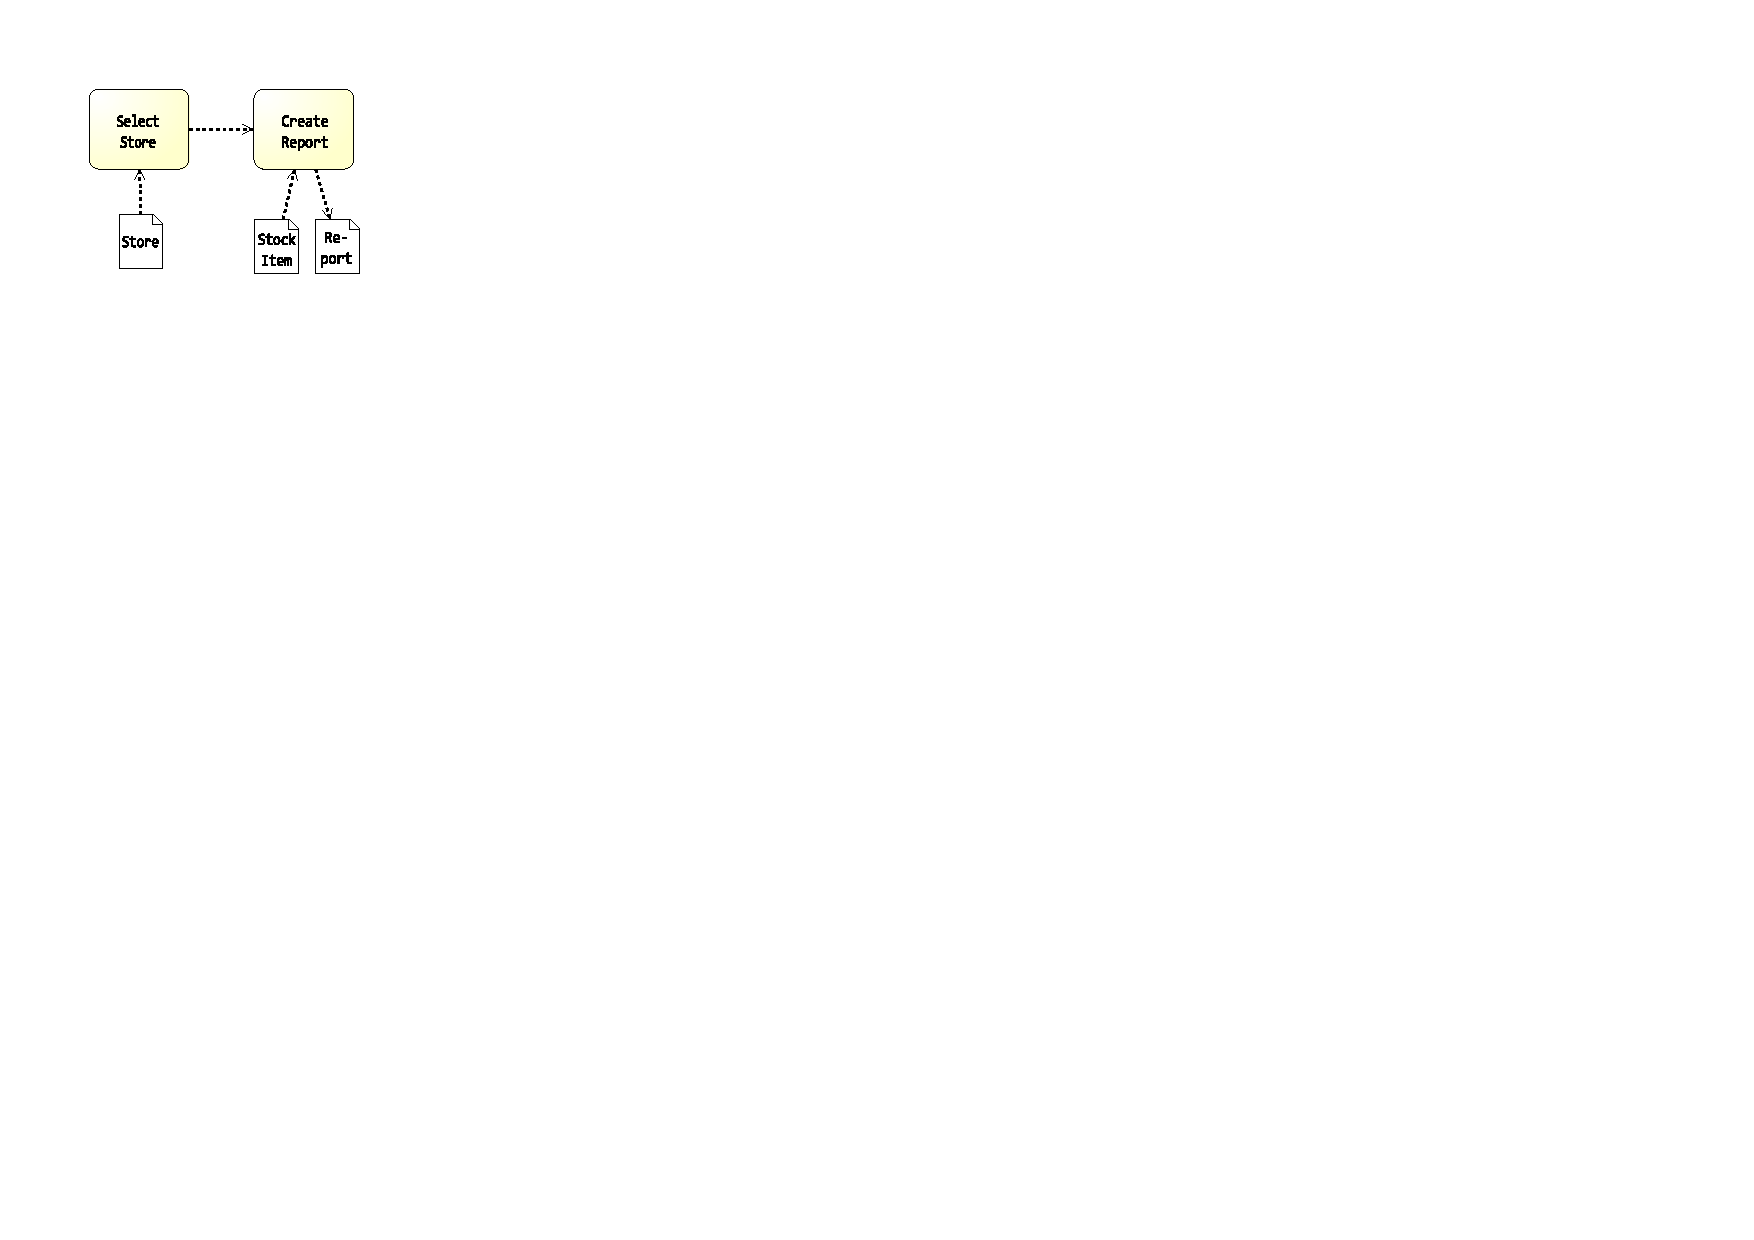
\includegraphics[width=5.5cm, trim={3cm 16cm 22cm 1cm}]{img/UC5DFD.pdf}
	\caption{Data Flow UC5 - Show Stock Reports }
	\label{fig:UC5DFD}
\end{figure}

%"l, b, r, t"
\begin{figure}[h!]
	\centering
	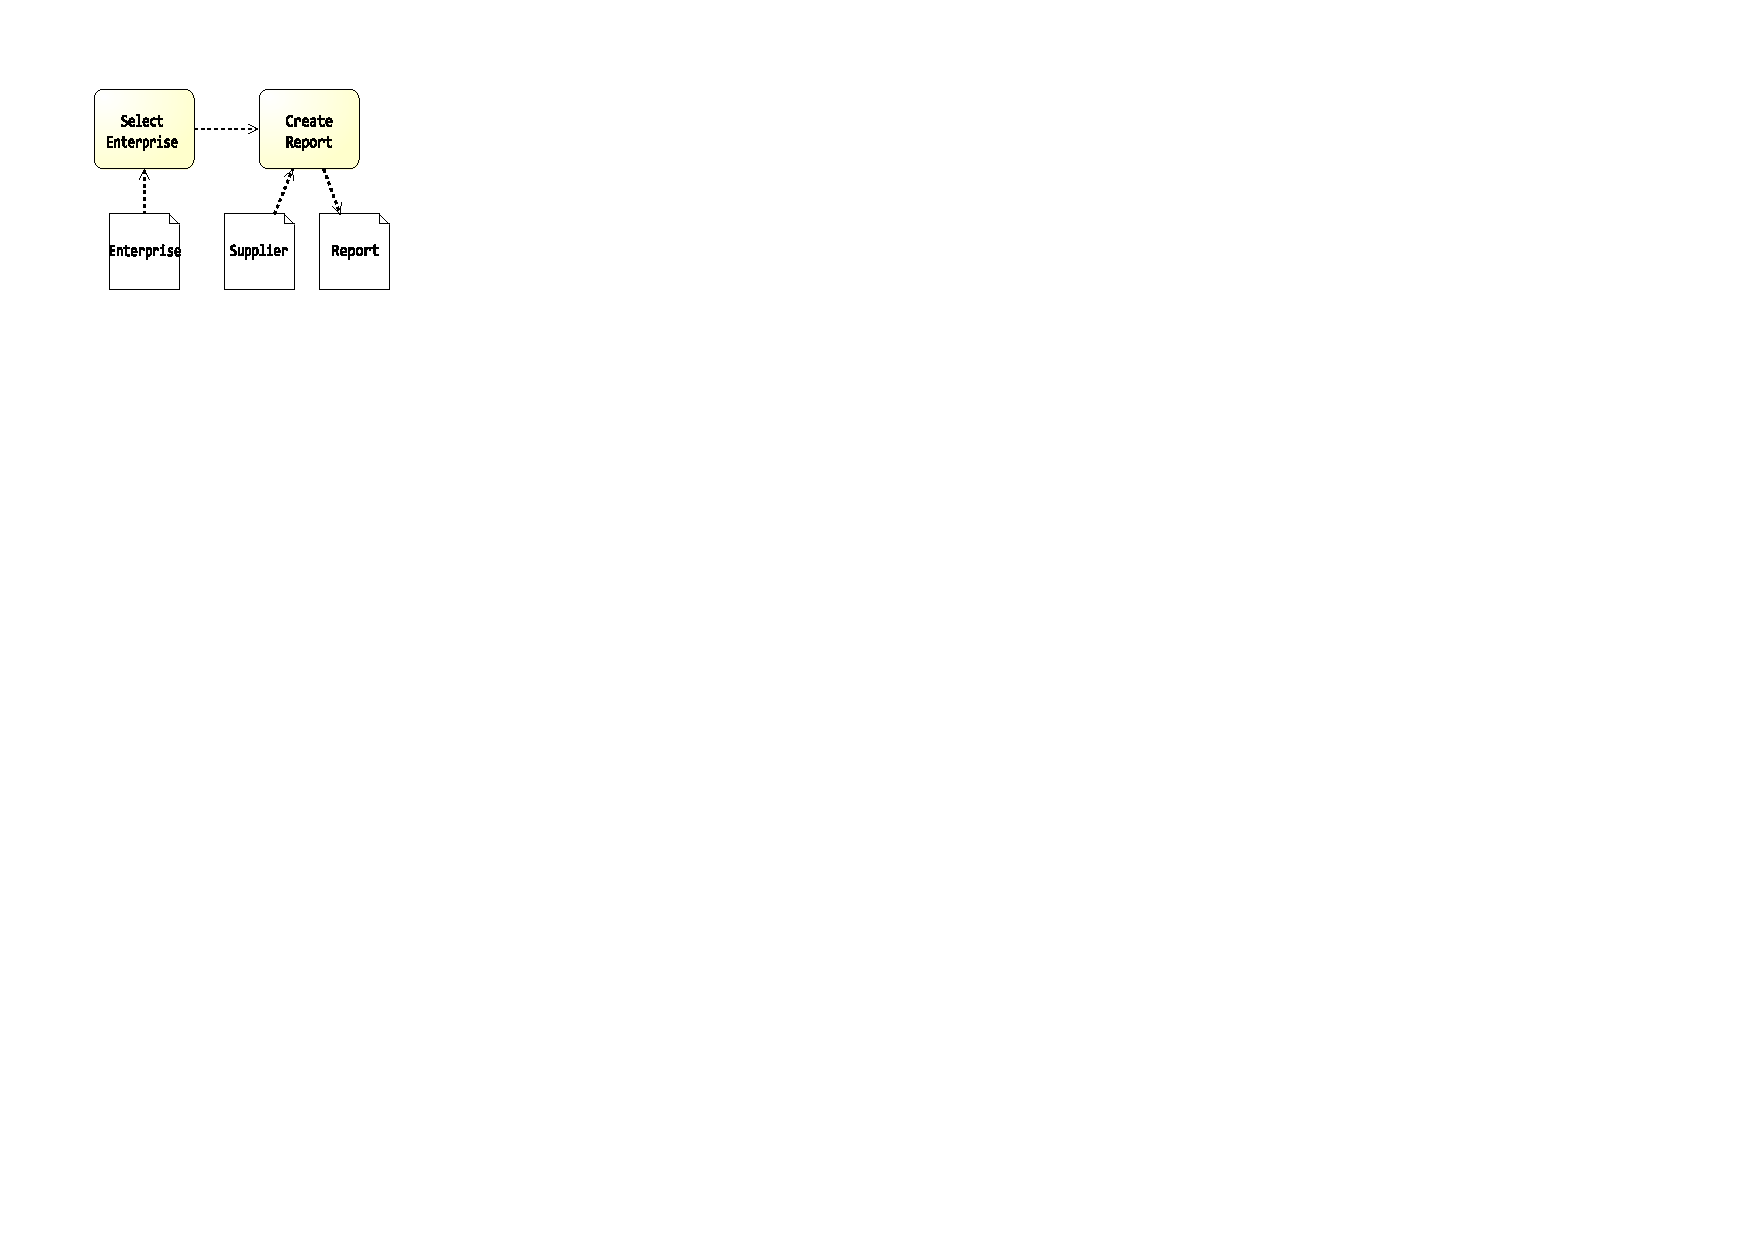
\includegraphics[width=5.5cm, trim={3cm 16cm 22cm 1cm}]{img/UC6DFD.pdf}
	\caption{Data Flow UC6 - Show Delivery Reports }
	\label{fig:UC6DFD}
\end{figure}

%"l, b, r, t"
\begin{figure}[h!]
	\centering
	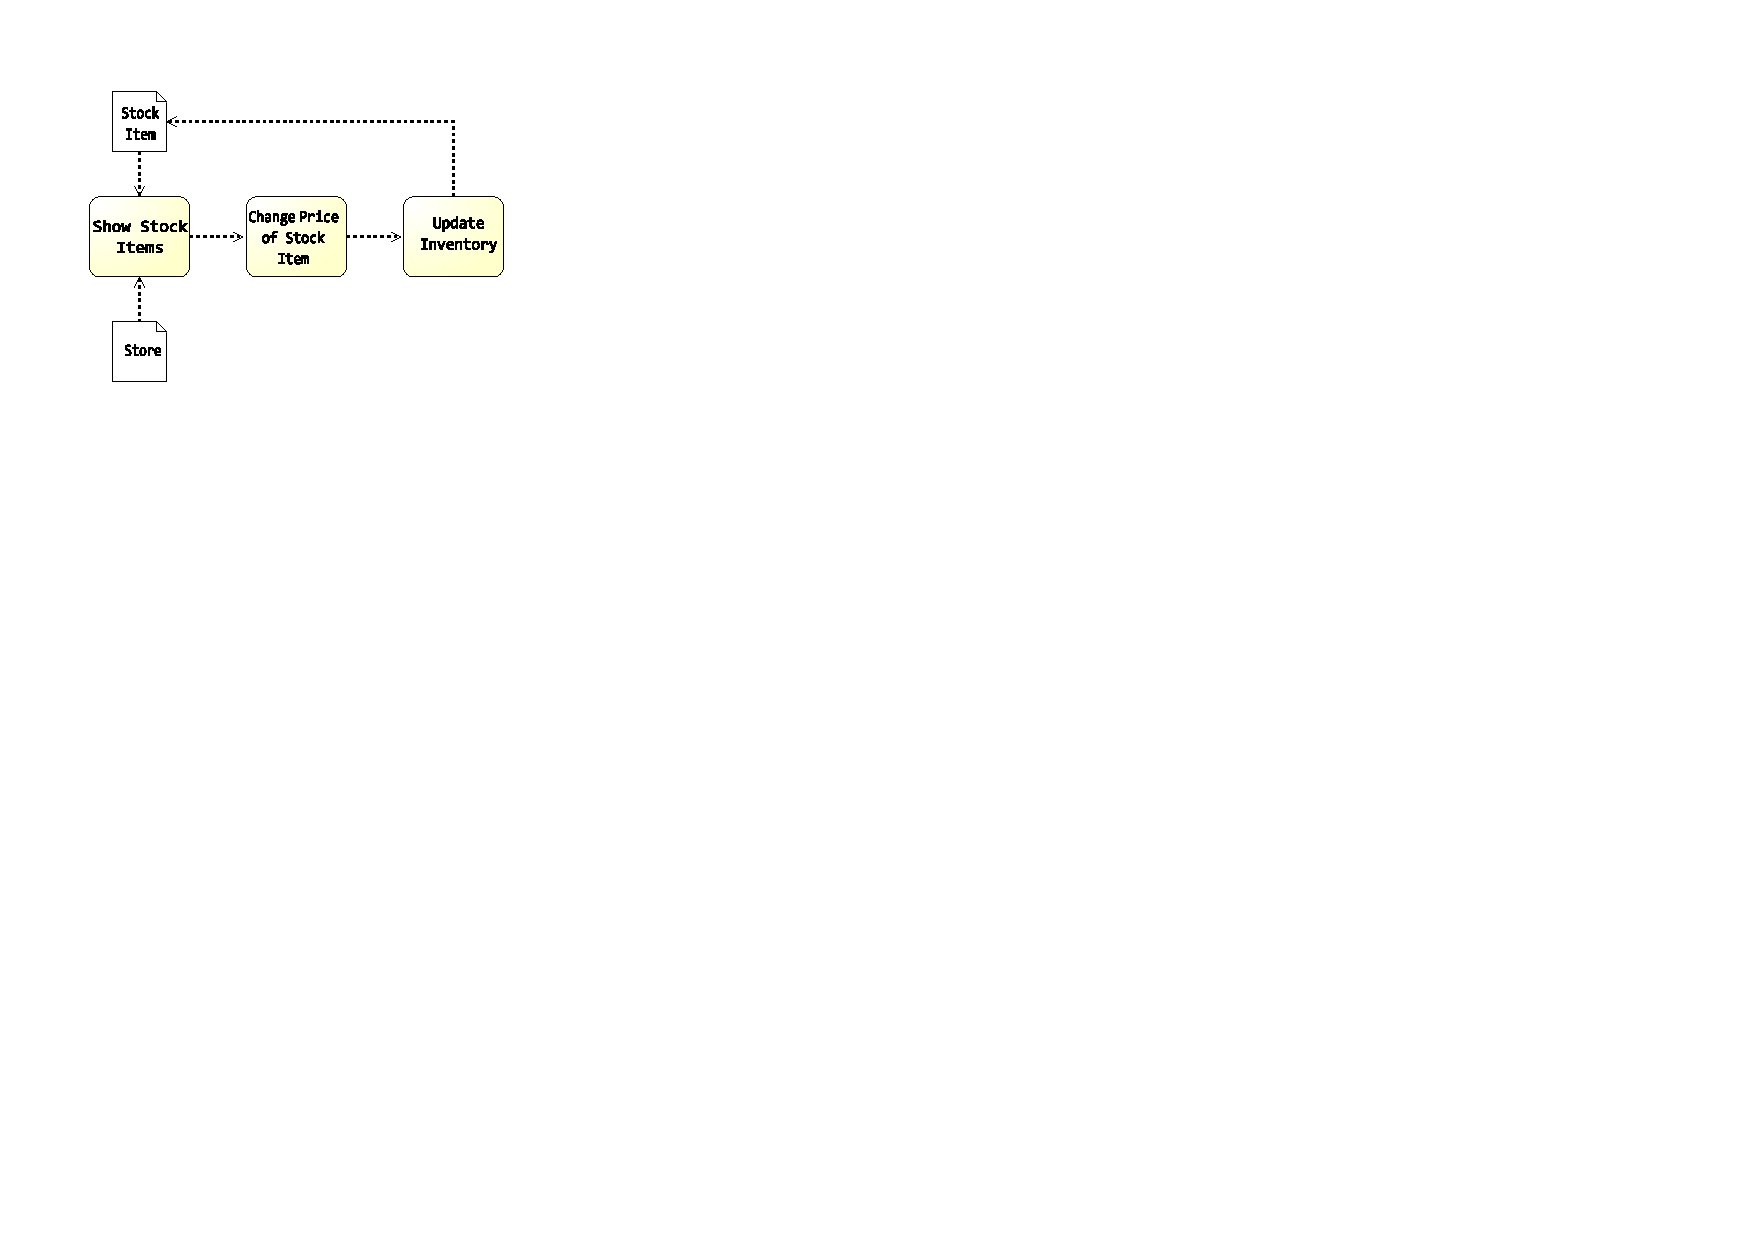
\includegraphics[width=5.5cm, trim={3cm 14.5cm 22cm 1cm}]{img/UC7DFD.pdf}
	\caption{Data Flow UC7 - Change Price }
	\label{fig:UC7DFD}
\end{figure}








\end{document}
